%\PassOptionsToPackage{draft}{graphicx} % to leave out images and speed up compiler

\documentclass[xcolor=svgnames]{beamer}
%\documentclass[xcolor=svgnames]{beamer}
%\includeonlyframes{current}

\usepackage[utf8]    {inputenc}
\usepackage[T1]      {fontenc}
\usepackage[english] {babel}

\usepackage{hyperref}
\hypersetup{
    colorlinks=true,
    linkcolor=blue,
    filecolor=magenta,      
    urlcolor=cyan,
}
\usepackage{url}

\newcommand{\btVFill}{\vskip0pt plus 1filll}


\setbeamertemplate{theorems}[numbered] 


\usepackage{amsmath,amsfonts,graphicx}
\usepackage{beamerleanprogress}
\usepackage{xcolor}
\usepackage{soul}
\usepackage{multicol}
\usepackage{tikz} 
\usepackage[export]{adjustbox}

\definecolor{iyellow}{RGB}{255, 162, 23}
\definecolor{sgreen}{RGB}{118, 191, 138}


\newcommand{\yellow}[1]{\textcolor{iyellow}{#1}}
\newcommand{\green}[1]{\textcolor{sgreen}{#1}}
\newcommand{\red}[1]{\textcolor{red}{#1}}
\newcommand{\blue}[1]{{\textcolor{blue}{#1}}}

\newcommand{\latered}[2]{\color<#2->{red}{#1}}

\newcommand{\cell}[1]{{\sf \textbf{\textcolor{DarkMagenta}{#1}}}}
\newcommand{\ra}{$\rightarrow$ }
\usetikzlibrary{shadows}

\newcommand*\keystroke[1]{%
  \tikz[baseline=(key.base)]
    \node[%
      draw,
      fill=white,
      drop shadow={shadow xshift=0.25ex,shadow yshift=-0.25ex,fill=black,opacity=0.75},
      rectangle,
      rounded corners=2pt,
      inner sep=1pt,
      line width=0.5pt,
      font=\scriptsize\sffamily
    ](key) {#1\strut}
  ;
}



\title
  [Data 301 Data Analytics\hspace{2em}]
  {Data 301 Data Analytics\\
  Spreadsheets: Microsoft Excel\\
  Part 2 of 3}

\author
  [Dr.\ Irene Vrbik]
  {Dr.\ Irene Vrbik}

\date
  {Term 1, 2019}

\institute
  {University of British Columbia Okanagan \newline irene.vrbik@ubc.ca}



\begin{document}


\graphicspath{{img/}}


\maketitle



\section
  {03ExcelPart2i.xlsx}



\begin{frame}{Charts}
A \emph{chart} is a graphical representation of spreadsheet data.\\[1em]

Charts can help you visualize relationships between data and create maximum impact on your audience. \\[1em]

When you create a chart, you can select from many chart types (eg, a stacked column chart or a 3-D exploded pie chart). \\[1em]

To create a line/bar/pic/etc. chart, the user to supply the data that will be displayed.\\[1em]
\end{frame}


\begin{frame}{Charts}
Once your data is selected, navigate to the {\bf Insert} tab, then click the desired {\bf Chart} Icon.  You can either choose one from the {\bf Recommended Chart} button or select from the variety of chart types.
 \begin{center}
%    \includegraphics[width=.6\textwidth]{chart1}
%        \includegraphics[width=.4\textwidth]{chart2}
    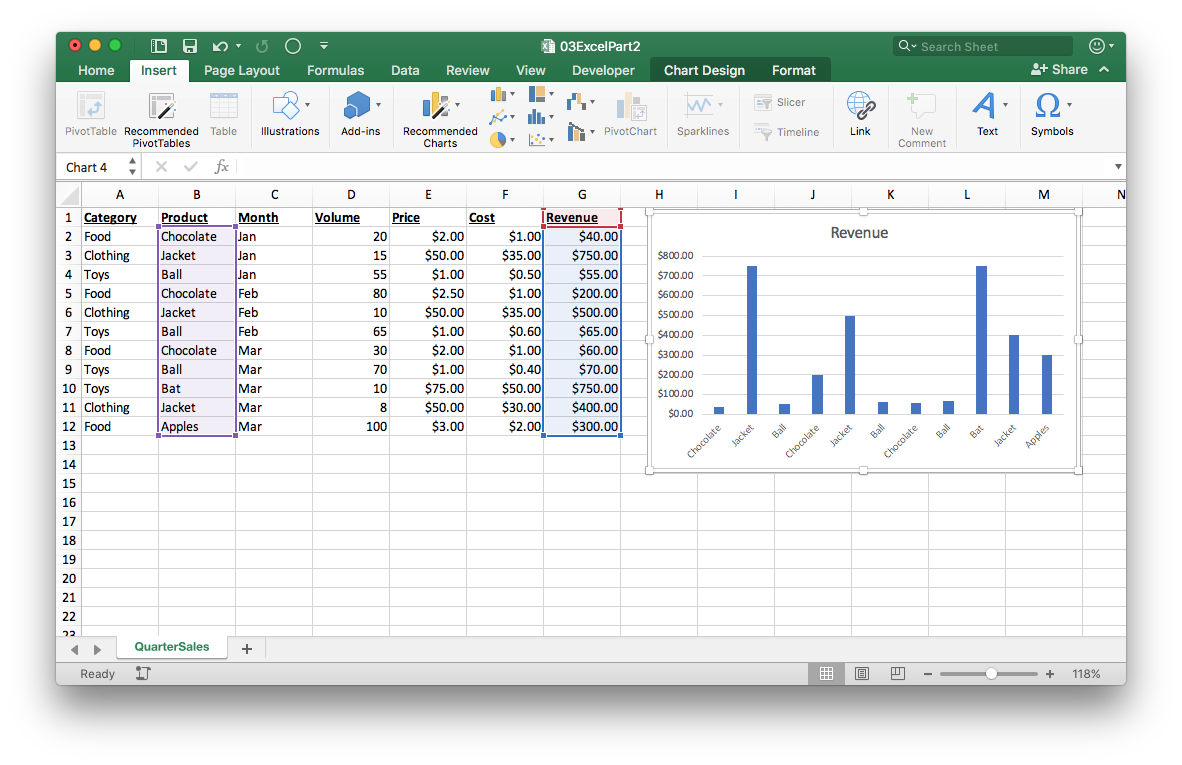
\includegraphics[width=.8\textwidth]{barchart}
 \end{center}
 \vspace{-1em}

\end{frame}

\begin{frame}
 Sometimes the default graphic is not what we want,\dots\\
 \medskip
 For instance the recommended chart on the previous page shows an individual bar for each instance of the product type.\\
 \medskip 
 We could instead create the total revenue for each product by selecting:
 \begin{itemize}
 \item The histogram icon 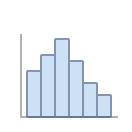
\includegraphics[height=1.5em]{histicon}
 \item Double clicking on the bars
 \item Selecting the Series Options icon: 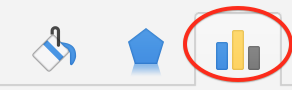
\includegraphics[height=1.5em]{seriesopt}
 \item Selecting {\it By Category} in the {\bf Bins} drop down menu.
 \end{itemize}
 
 \end{frame}


\begin{frame}{Chart Options}
After you create a chart, you can customize it by applying chart quick layouts or styles.  The
\textbf{Chart Design} tab also provides a number of features for modifying things like chart color/type/position/etc.
 \begin{center}
%    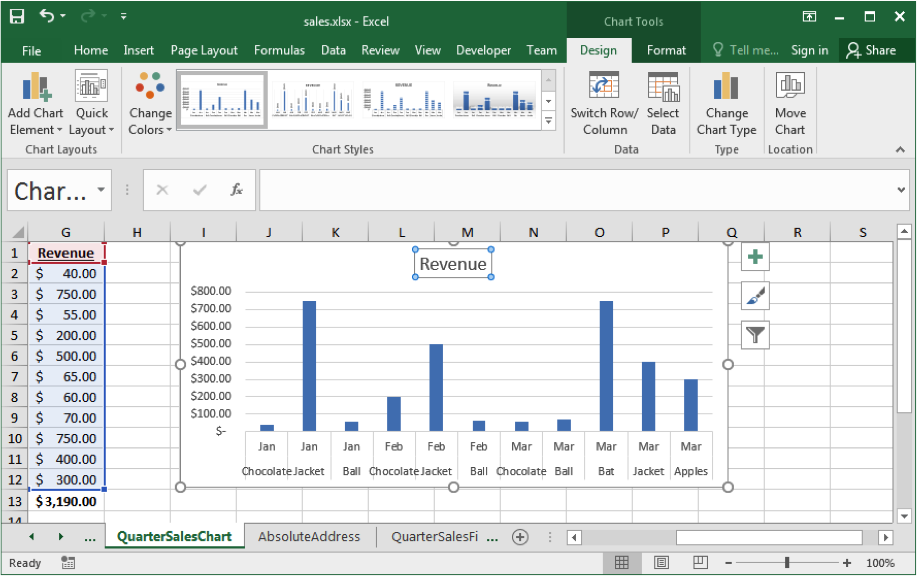
\includegraphics[width=.8\textwidth]{ChartTools}
  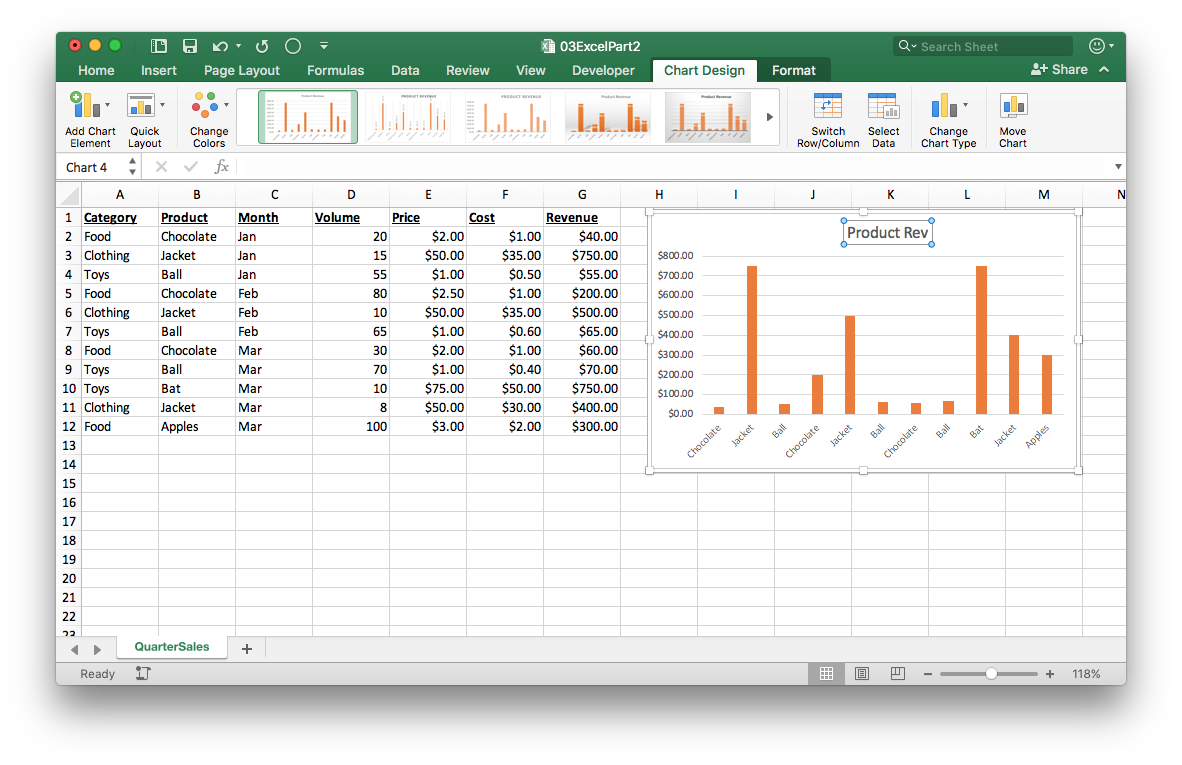
\includegraphics[width=.8\textwidth]{ChartTools2}
 \end{center}

\end{frame}


\begin{frame}{Chart Options}
\begin{example}
Navigate to the {\bf Chart Design} tab and relocate your chart to a new worksheet called \textit{barchart}. 
\end{example}
 \begin{center}
  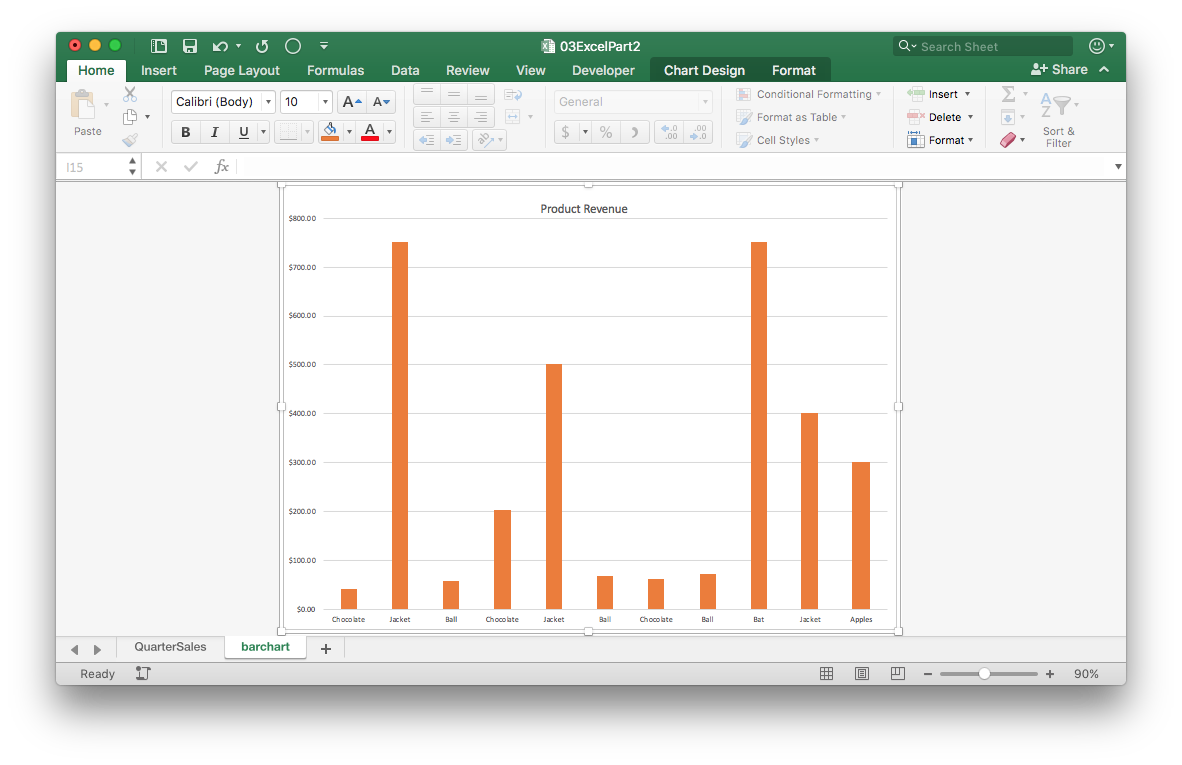
\includegraphics[width=.8\textwidth]{barcharttab}
 \end{center}
\end{frame}


\begin{frame}{Trendlines}
\begin{itemize}
\item Trendlines can be easily added to a number of  chart types.  
\item  Click on chart, "Add Chart Element"...."Trendline"
\end{itemize}
 \begin{center}
  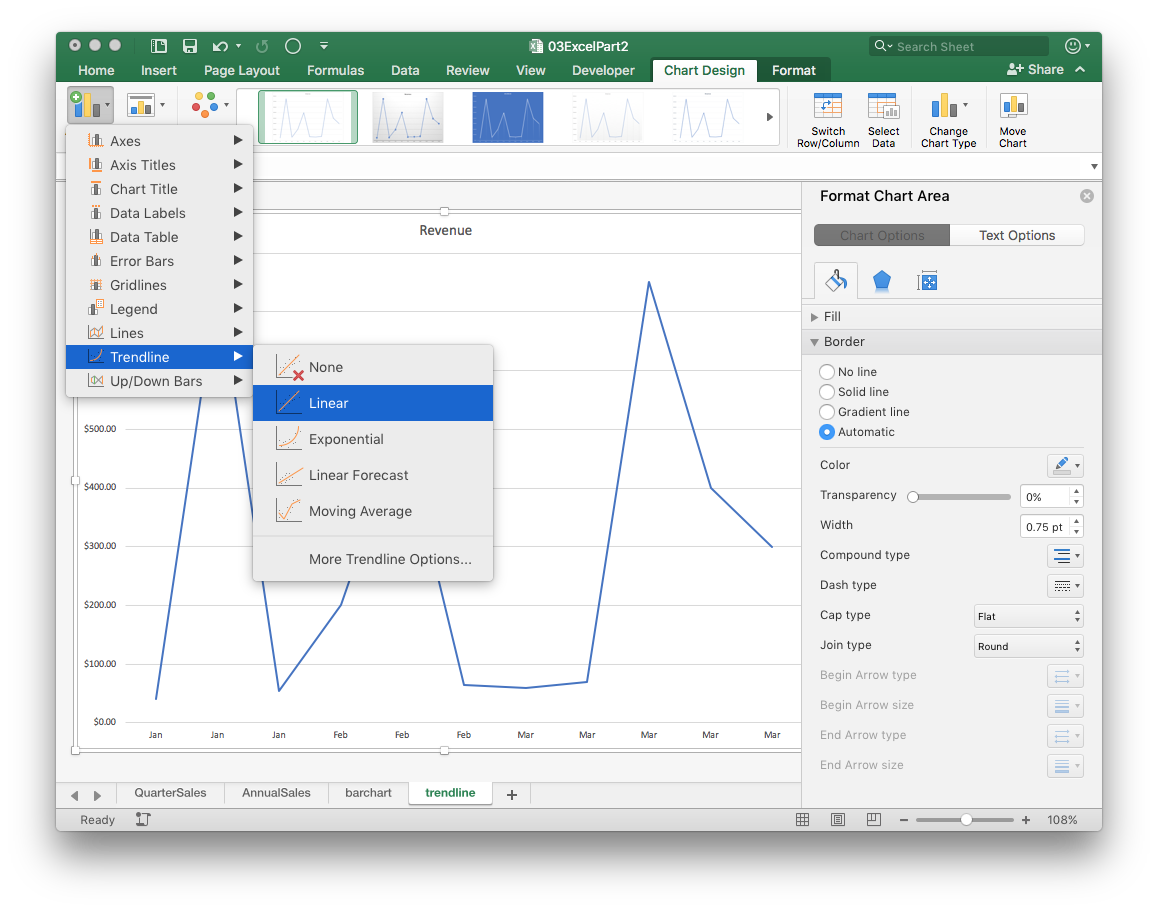
\includegraphics[width=.8\textwidth]{trendline}
 \end{center}
% A a linear trendline a good choice here?
\end{frame}




\begin{frame}{Trendlines}
Trendlines can be easily added to any chart.
\begin{itemize}
\item Linear treadline for monthly revenue.  Good choice?
\end{itemize}
\begin{columns}[T] % align columns
\begin{column}{.48\textwidth}
\vspace{5mm}
 \begin{center}
 \hspace*{6mm}                                                           
    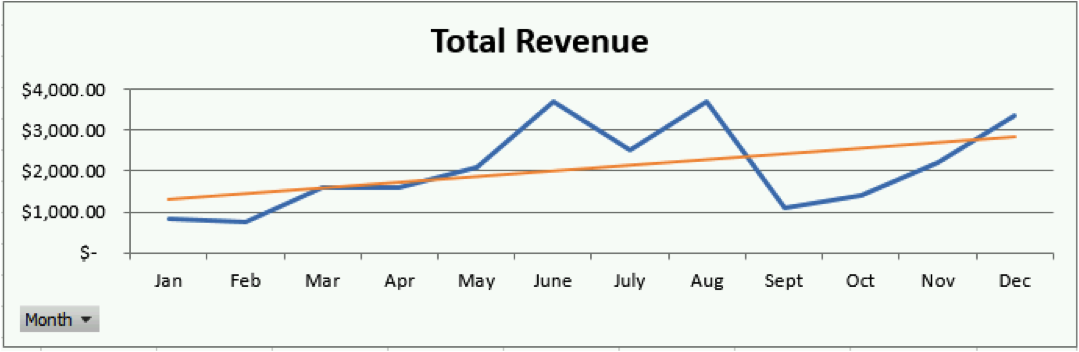
\includegraphics[width=1.3\textwidth]{Trendlines1}
 \end{center}
  \begin{alertblock}{}
Probably not, as data appears to be seasonal  \end{alertblock}
\end{column}%
\hfill%
\begin{column}{.48\textwidth}
\vspace{-5mm}
 \begin{center}
        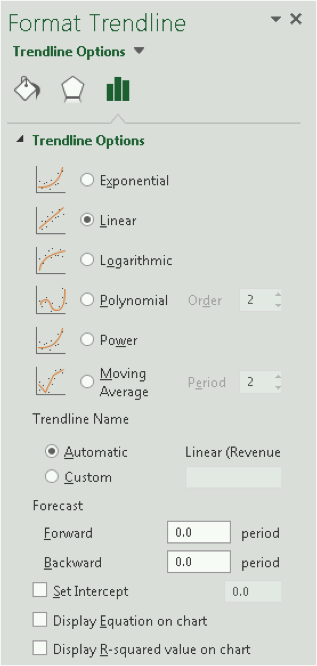
\includegraphics[height=.7\textheight]{Trendlines2}
 \end{center}
\end{column}%
\end{columns}
\end{frame}

\begin{frame}{Try it! Trendline}
Of course it wouldn't really make sense to add a linear trend to the previous line chart since the data do not appear linear.
\begin{exampleblock}{Apples}
\begin{enumerate}
\item Create a line chart that plots the revenue per month for only {\bf Apples} using the {\bf Annual Sales data}. 
\item Add a linear trendline.
\item In {\bf Chart Design} tab, select a design that displays the months on a 45 degree angle. 
\end{enumerate}
\end{exampleblock}
\end{frame}


\begin{frame}{Try It: Chart}
\begin{exampleblock}
{Question:}  Create a Pareto chart (option under the histogram icon) to make it easy to see the best selling product.
\end{exampleblock}
 \begin{center}
        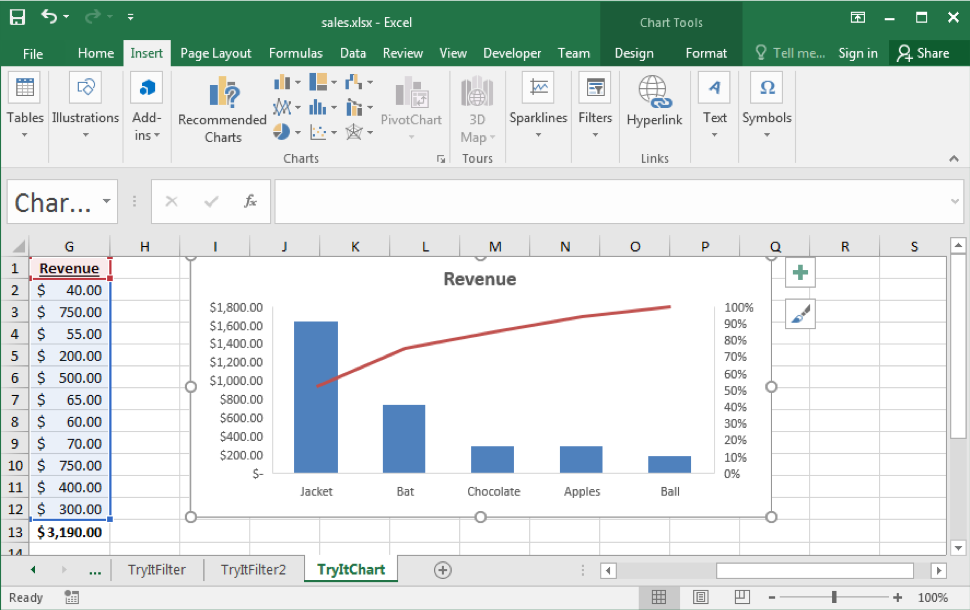
\includegraphics[width=.8\textwidth]{pareto}
 \end{center}
% \red{BLAH come back to example when you have the latest version of Microsoft Office.}
\end{frame}

\begin{frame}{Sparklines}
A \emph{sparkline} is a tiny chart in a worksheet cell for a quick data overview.
\begin{itemize}
\item Click {\bf Insert} then select {\bf Sparklines\dots} 
\item Displayed below is an example of a \textit{line} and \textit{column} sparkline.
\item You can change the style in the {\bf Sparkline} tab in the ribbon.
\end{itemize}
 \begin{center}
        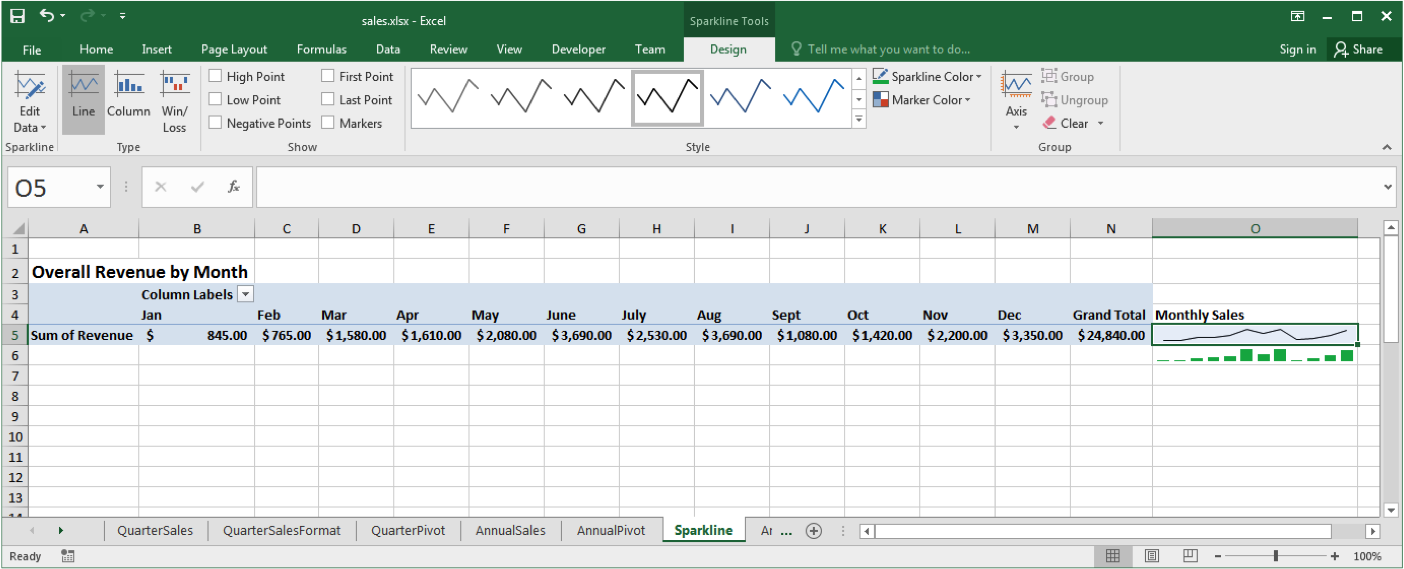
\includegraphics[width=.9\textwidth]{Sparklines}
 \end{center}
\end{frame}





\begin{frame}{Pivot Tabels}
\emph{Pivot tables} allow for easily aggregating and exploring large data sets.\\[1em]
\begin{itemize}
\item For example, our data set can be summarized by revenue by month.
\end{itemize}
\begin{center}
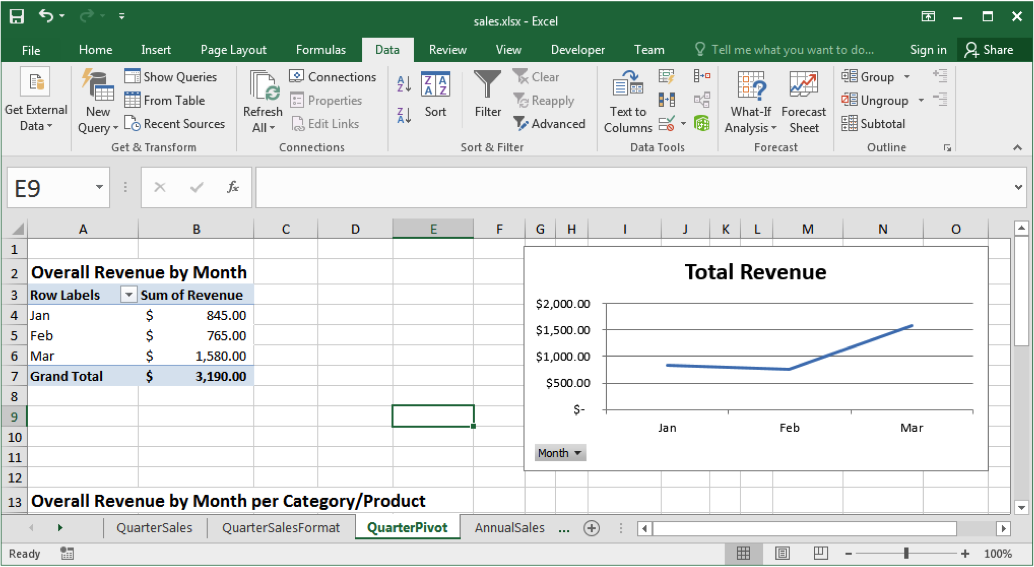
\includegraphics[width=0.8\textwidth]{pivot}
\end{center}
\end{frame}


\begin{frame}{Creating a Pivot Table}
To create a pivot table
\begin{enumerate}
\item Select the data (or click any single cell inside the data set).
\item  Navigate to the {\bf Insert} tab, select the drop down {\bf Tables} menu, and click the PivotTable icon. 
\item Click OK
\item Add fields in the PivotTable Fields pane
\end{enumerate}
{\bf Drag fields}
To get the total revenue for each month, drag the following fields to the different areas.
\begin{enumerate}
\item  {\tt Month} to the Rows area.
\item {\tt Revenue} to the  Values area.
\end{enumerate}
\end{frame}

% Dates aren't in order in Annual Sales (that's because June, July and Sept are in the wrong format-- need Jun, Jul, Sep)
% side note: https://answers.microsoft.com/en-us/msoffice/forum/all/pivot-table-sort-by-month/923b6ffa-9ad3-4885-9c3c-e5f4360a44d1
% https://contexturesblog.com/archives/2011/09/30/excel-pivot-table-sorting-problems/

\begin{frame}{Creating a Pivot Table}
The following dialog box appears. Excel automatically selects the data for you. The default location for a new pivot table is New Worksheet.

\begin{center}
\begin{tikzpicture}
%  \node (img1) {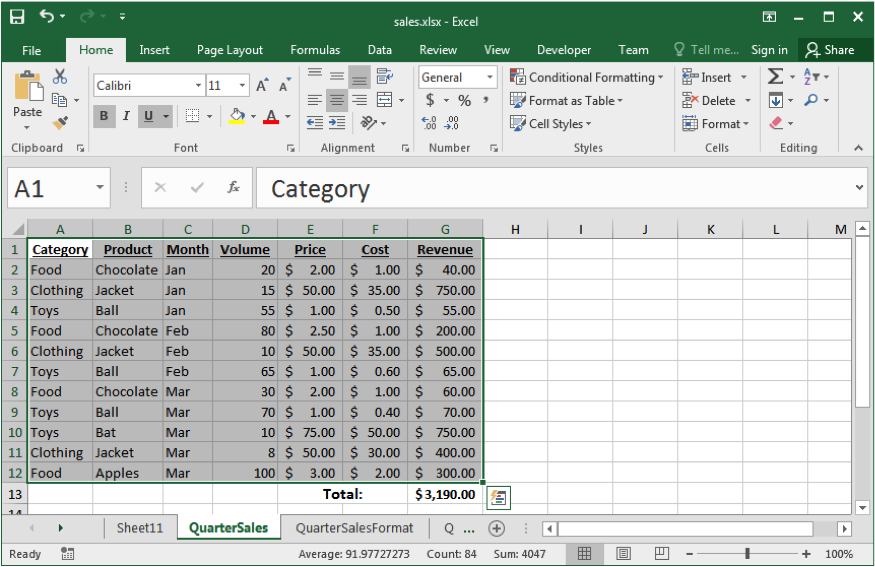
\includegraphics[width=0.9\textwidth]{pivot1}};
  \node (img1) {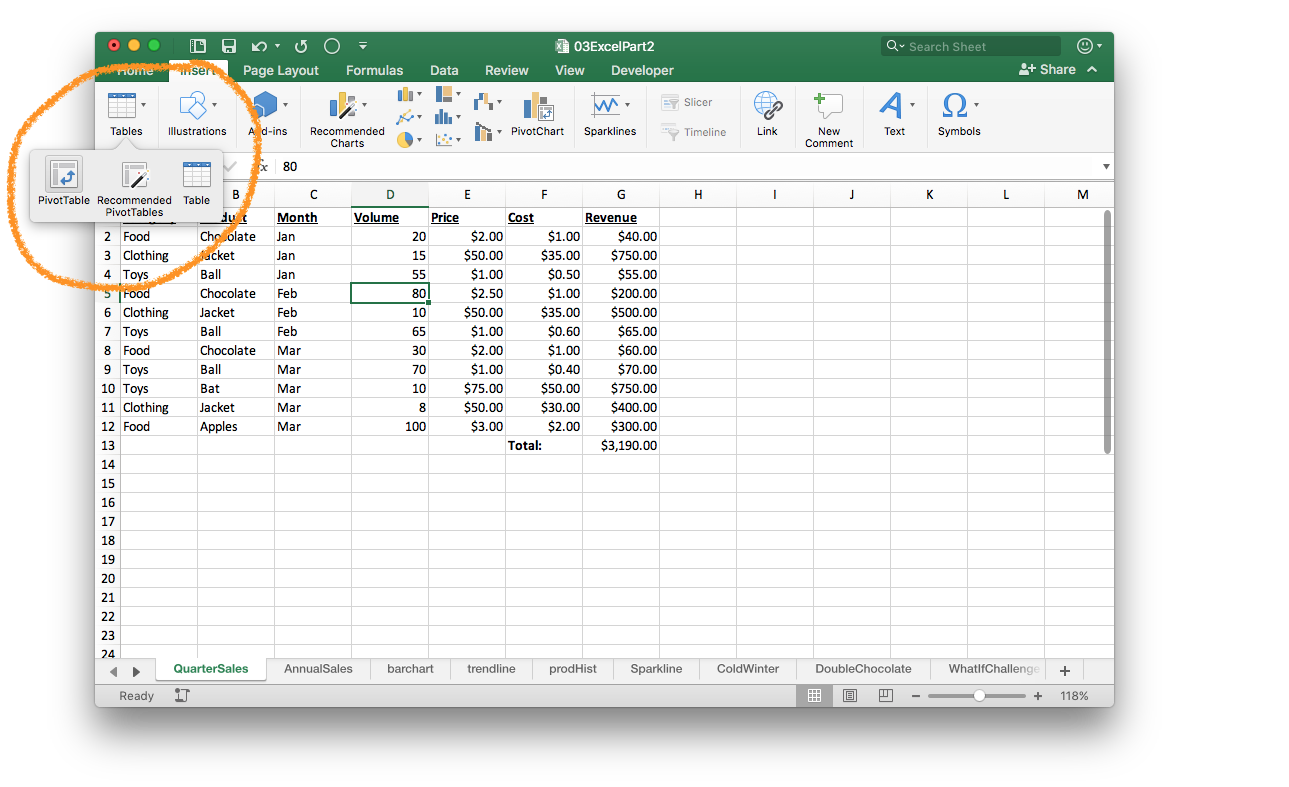
\includegraphics[width=0.9\textwidth]{pivotOne}};
  \node (img2) at (img1.east) [xshift=-2cm] %{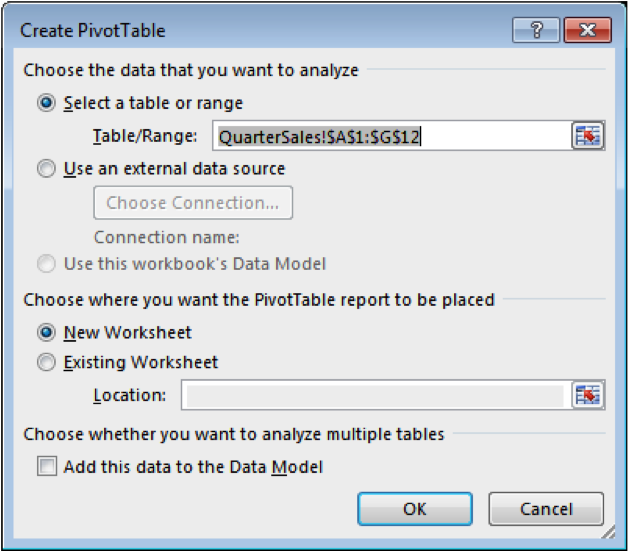
\includegraphics[height=5cm]{pivot2}};
{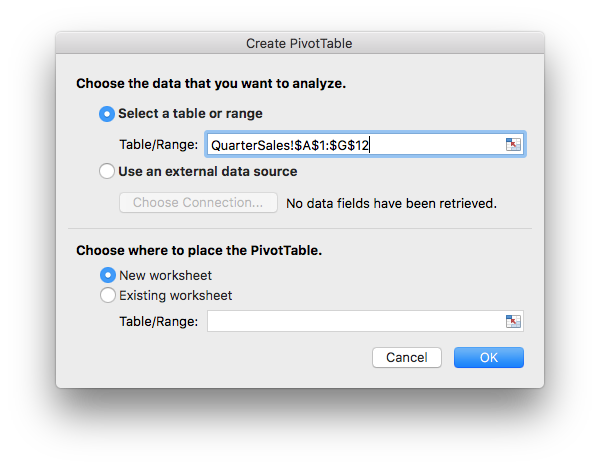
\includegraphics[height=5cm]{pivotTwo}};
\end{tikzpicture}
\end{center}
\end{frame}


\begin{frame}{Creating a Pivot Table}
\begin{columns}[T] % align columns
\begin{column}{.48\textwidth}
\textit{Pivot1} worksheet
{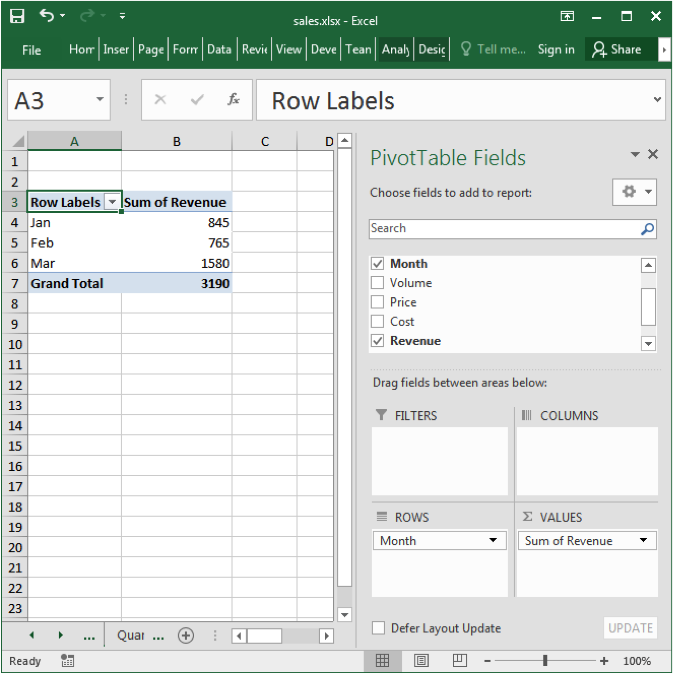
\includegraphics[width=1.2\textwidth]{pivot3}}
\end{column}%
\hfill%
\begin{column}{.48\textwidth}
\vspace{1em}
Add fields to pivot table.\\[1em]
Field may either be:
\begin{itemize}
\item ROWS value
\item  COLUMNS value
\item  Cell VALUES (aggregated)
\item  Used in a FILTERS (we could also filter using the drop down filter option; select the dropdown arrow located in cell A3, for example)
%\item \alert{Notice:} if we filter out the month of January using the drop down filter, it will still contribute to the Grand Total. NOT TRUE
\end{itemize}
\end{column}%
\end{columns}
N.B Right click on a cell in the pivot table and select Show/Hide Fields List to show/hide the pop-up window on the right.
\end{frame}

\begin{frame}{Pivot Table Example}
\begin{columns}[T] % align columns
\begin{column}{.48\textwidth}
\textit{Pivot2} worksheet
{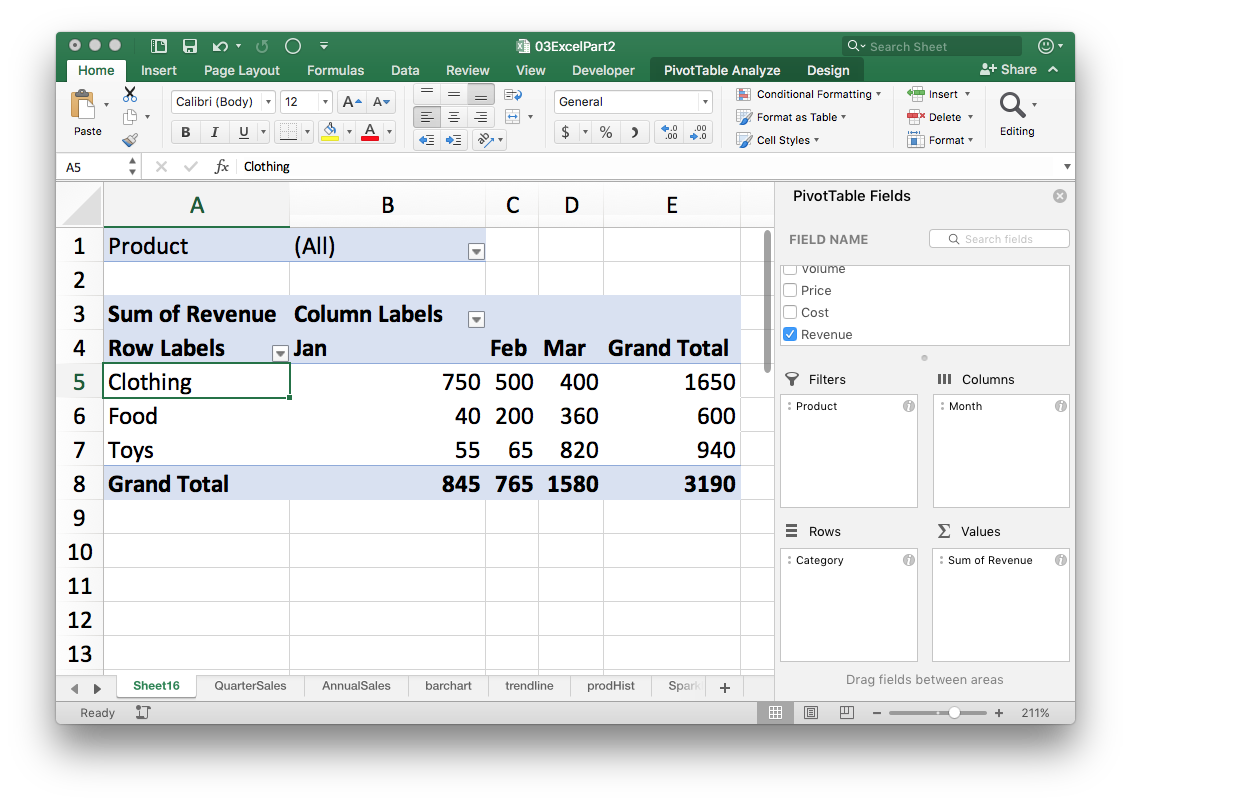
\includegraphics[width=1.2\textwidth]{pivotExample}}
\end{column}%
\hfill%
\begin{column}{.48\textwidth}
\vspace{1em}
\begin{itemize}
\item Categories are rows.
\item Months are columns.
\item Each cell is a sum of revenue per category for that month.
\item We can filter on product (eg. filter out apples).
\end{itemize}
\end{column}%
\end{columns}
\end{frame}

\begin{frame}{Pivot Table Example}
\begin{columns}[T] % align columns
\begin{column}{.48\textwidth}
\textit{Pivot3} worksheet
{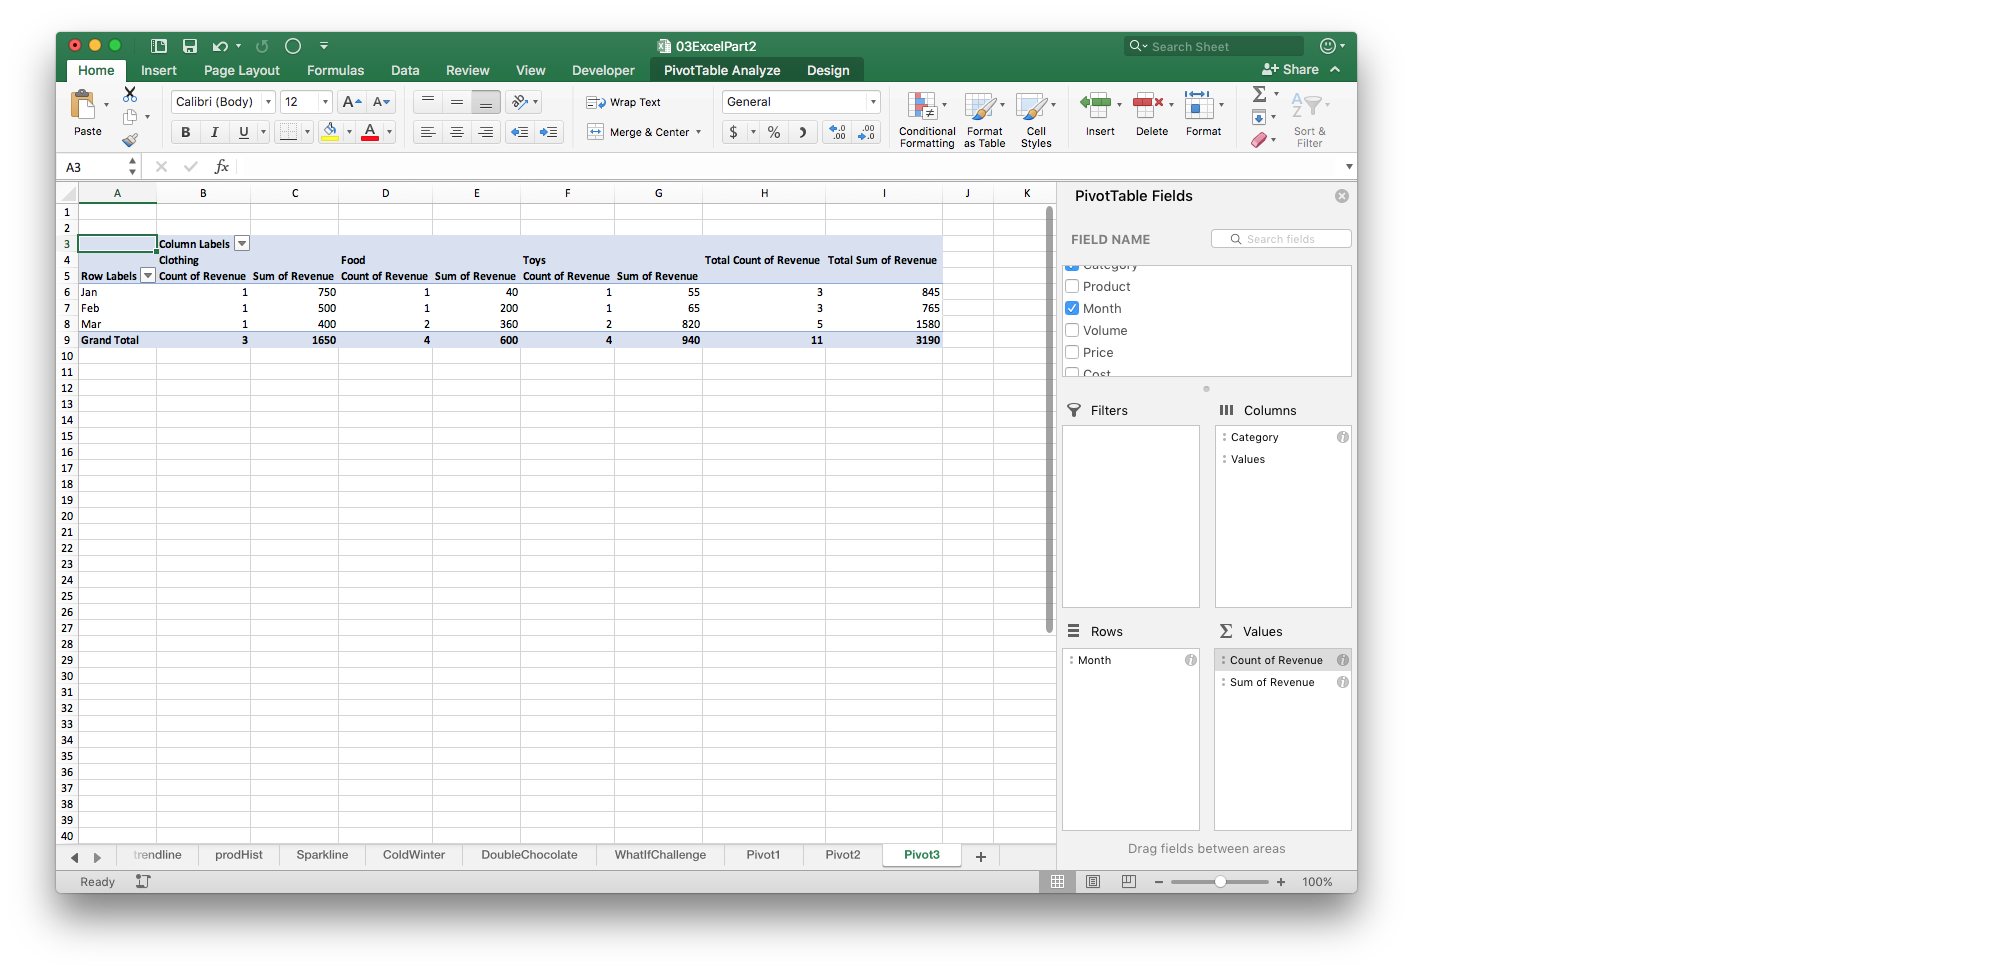
\includegraphics[width=1.8\textwidth]{pivotThree}}
\end{column}%
\hfill%
\begin{column}{.48\textwidth}
\vspace{1em}
\begin{itemize}
\item Notice that the same field can be used in VALUES multiple times
\item In that way we can see multiple aggregate summaries (eg. total and count)

\item To change the value aggregation function, click on the  
\includegraphics[width=1em]{img/i.png}\ icon
\item Notice that a field can NOT be used in ROWS/COLUMNS/FILTER at the same time.
\end{itemize}
\end{column}%
\end{columns}
\end{frame}



\begin{frame}{Try It: Pivot Table}
\begin{exampleblock}{Question:} Create a pivot table using the annual sales data that shows the total revenue per month by category/product. 
\end{exampleblock}
\begin{center}
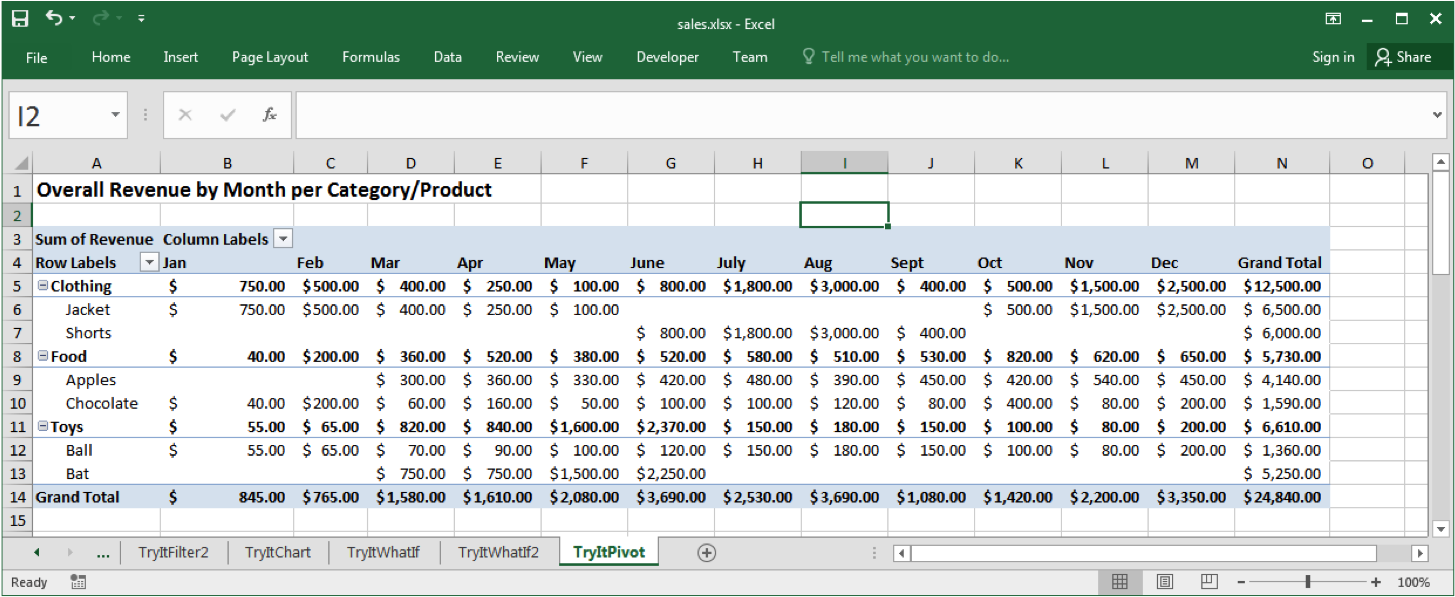
\includegraphics[width=.9\textwidth]{TryItPivot.png}
\end{center}
N.B. The order in which your fields appear in ROWS will make a difference.  Also, we can reformat the cells to display in {\bf currency} format.
\end{frame}

\begin{frame}{Pivot Charts}
A pivot chart is a chart attached to a pivot table.  Create it under {\bf Insert} then {\bf Pivot Chart}.
\begin{center}
%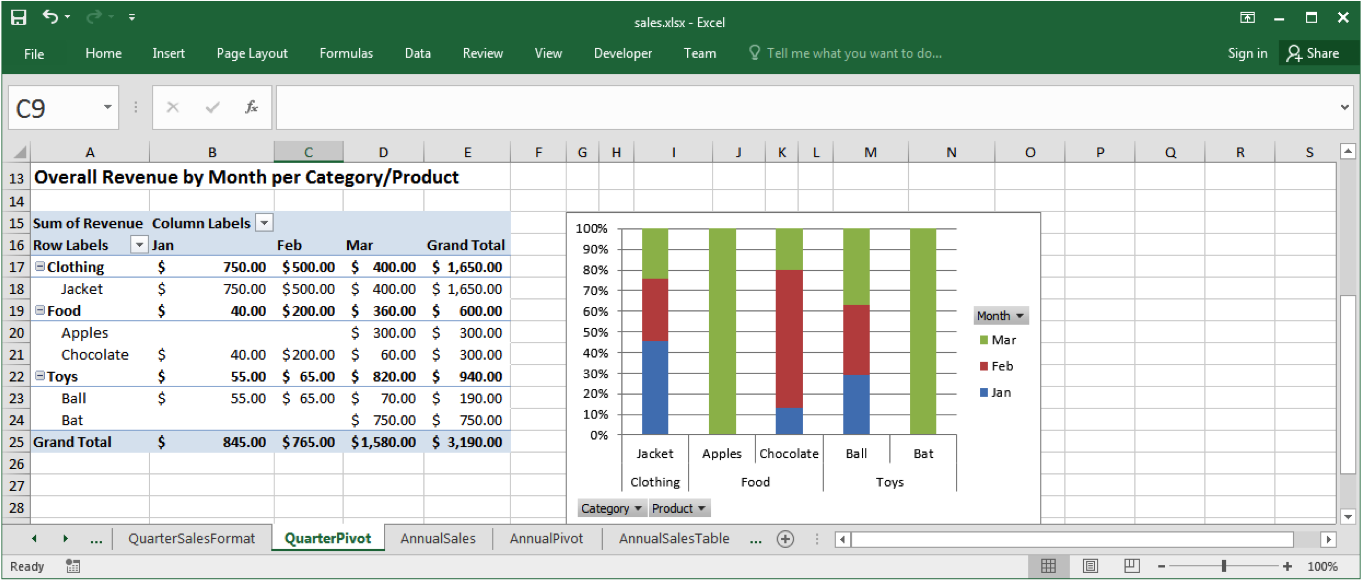
\includegraphics[width=.9\textwidth]{PivotChart.png}
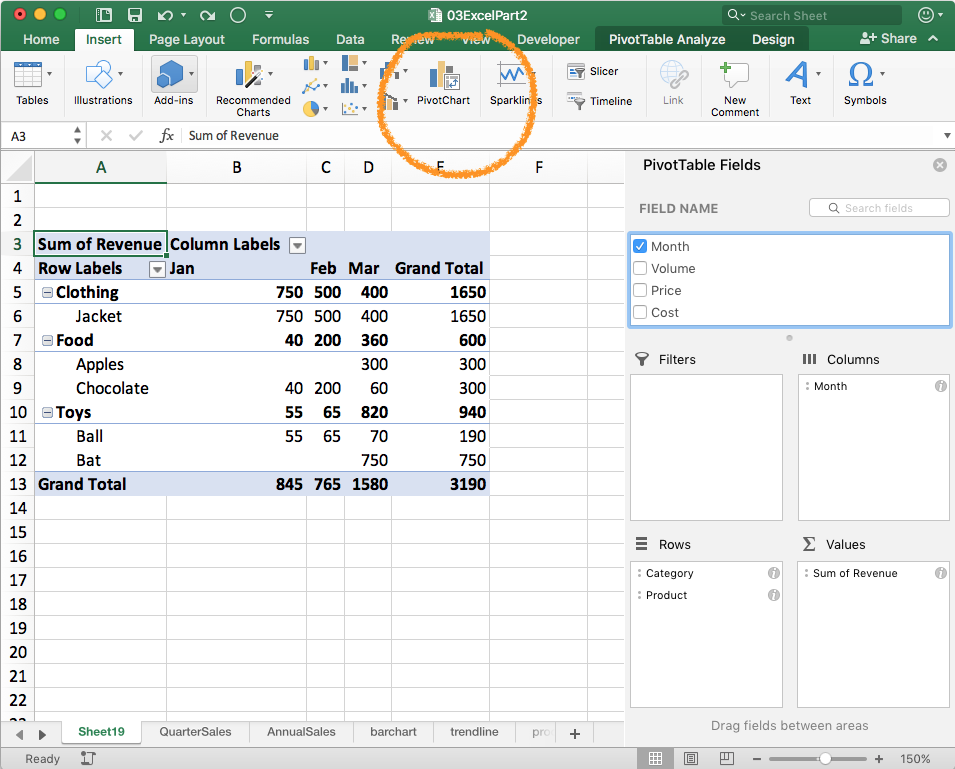
\includegraphics[width=.9\textwidth]{pivChart.png}
\end{center}
\end{frame}


\begin{frame}{Pivot Charts}
Below we have chosen a 100\% stacked bar chart type.
\begin{center}
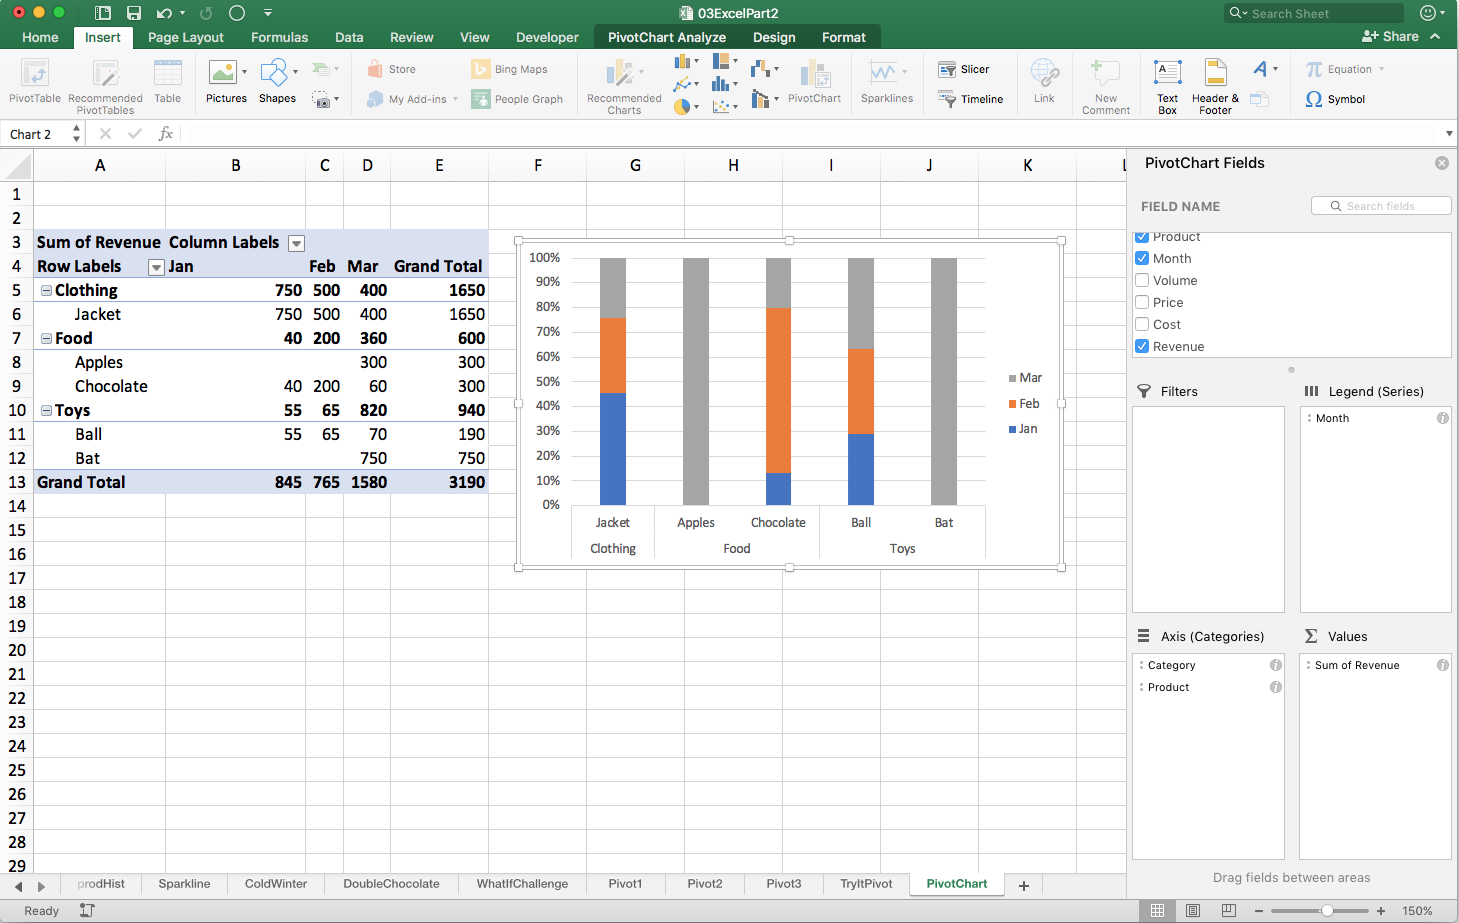
\includegraphics[width=.9\textwidth]{pivChart2.png}
\end{center}
\end{frame}




\begin{frame}{Pivot Tables Question}
  \begin{example}
 How many of the following statements are TRUE?
 \begin{enumerate}
%\item We can only change a single cell in a what-if scenario.
\item A pivot table field can be used in ROWS and COLUMNS at the same time.
\item A pivot table field can be used in VALUES more than once.
\item In our sales spreadsheet example, if Product and Category are both used in ROWS then the order they are list does not matter.
%\item It is not possible for a field that is a string to be used in VALUES.
 \end{enumerate}
\begin{multicols}{5}
\begin{enumerate}[A)]
\item 0 
\item 1
\item 2
\item 3
%\item 4
\end{enumerate}
\end{multicols}
  \end{example} 
\end{frame}

\begin{frame}<handout:0>{What-If and Pivot Tables Question}
  \begin{block}{Answer:}
 How many of the following statements are TRUE?
 \begin{enumerate}
%\item {\color<1->{red}{We can only change a single cell in a what-if scenario.}}
\item {\color<1->{red}{A pivot table field can be used in ROWS and COLUMNS at the same time.}}
\item {\color<2->{ForestGreen}{A pivot table field can be used in VALUES more than once.}}
\item {\color<3->{red}{In our sales spreadsheet example, if Product and Category are both used in ROWS then the order they are list does not matter.}}
%\item {\color<5->{red}{It is not possible for a field that is a string to be used in VALUES.}}
 \end{enumerate}
\begin{multicols}{5}
\begin{enumerate}[A)]
\item 0 
\item \textbf<4>{\textit<4>{{\color<4>{iyellow}{1}}}}
\item 2
\item 3
%\item 4
\end{enumerate}
\end{multicols}
  \end{block} 
\end{frame}


\section
  {03ExcelPart2ii.xlsx}


\begin{frame}{Conditions and Decisions}
A \emph{condition} is an expression that is either TRUE or FALSE.\\[1em]
Conditions are used to make decisions and perform different actions depending on the condition value.\\[1em]

Excel condition and decision functions:
\begin{description}
\item[{\tt FALSE()}]  returns {\tt FALSE}
\item[{\tt TRUE()}] returns {\tt TRUE}
\item[{\tt AND(cond1, cond2)}] returns {\tt TRUE} if both {\tt cond1} and {\tt cond2} are true
\item[{\tt OR(cond1, cond2)}] returns {\tt TRUE} if either or both of {\tt cond1} and {\tt cond2} are true
\item[{\tt NOT(cond)}] returns {\tt TRUE} if {\tt cond} is {\tt FALSE}
\end{description}
\end{frame}

\begin{frame}[fragile]{Decisions using {\tt IF()}}
 The {\tt IF()} function is used to make a decision based on a condition
\begin{itemize}
\item \verb|IF(condition, value_if_true, value_if_false)|
\end{itemize}
\medskip
 Example: If cell \cell{A2} is less than 5, return 10 otherwise return 20.
\begin{itemize}
\item \verb|= IF(A2 < 5, 10, 20)|
\end{itemize}
\medskip
If the third argument is not specified, it's default  is {\tt FALSE()}
\begin{itemize}
\item \verb|= IF(A2 < 5, 10)| returns {\tt FALSE()} if \cell{A2} is $\geq 5$
\end{itemize}
\medskip
The following statements are equivalent
\begin{itemize}
\item \verb|= IF(A2 < 5, TRUE(), FALSE())| same as \verb|=A2 < 5|
\end{itemize}
Hence if we just want to check if a condition is met, we don't need the {\tt IF()} function.

%\begin{center}
%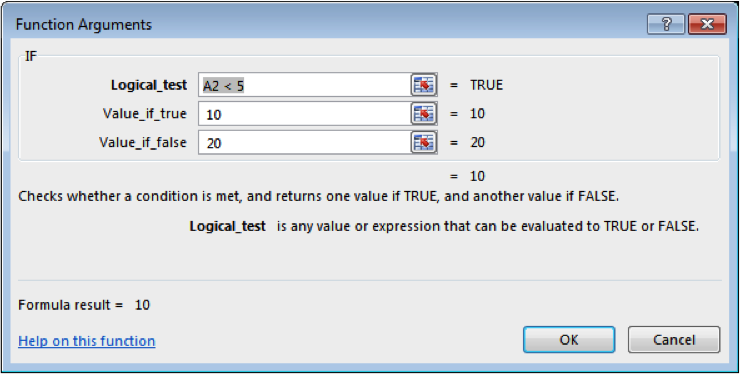
\includegraphics[width=.9\textwidth]{if.png}
%\end{center}
\end{frame}

\begin{frame}{Try it: {\tt IF()}}
\begin{exampleblock}{}{Question: Create two conditions:}
\begin{enumerate}
\item If cell \cell{B2} $\leq 10$, then show \cell{C2}, otherwise \cell{D2}.
\item If cell  \cell{B2}$ < 15$ and \cell{C2}$ > 20$, return \cell{B2}*\cell{C2}, otherwise if \cell{D2} $ < 10$, return 1, else 4.
\end{enumerate}
\end{exampleblock}
\begin{center}
%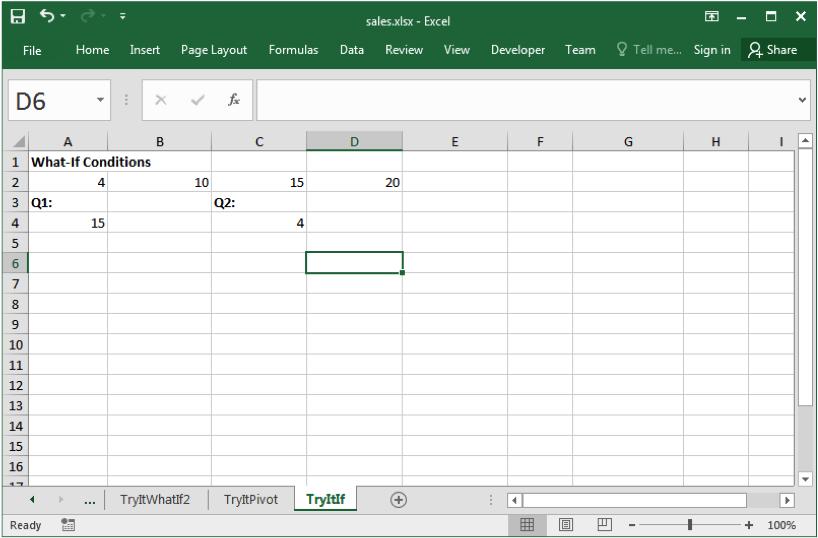
\includegraphics[width=.9\textwidth]{TryItIf.png}
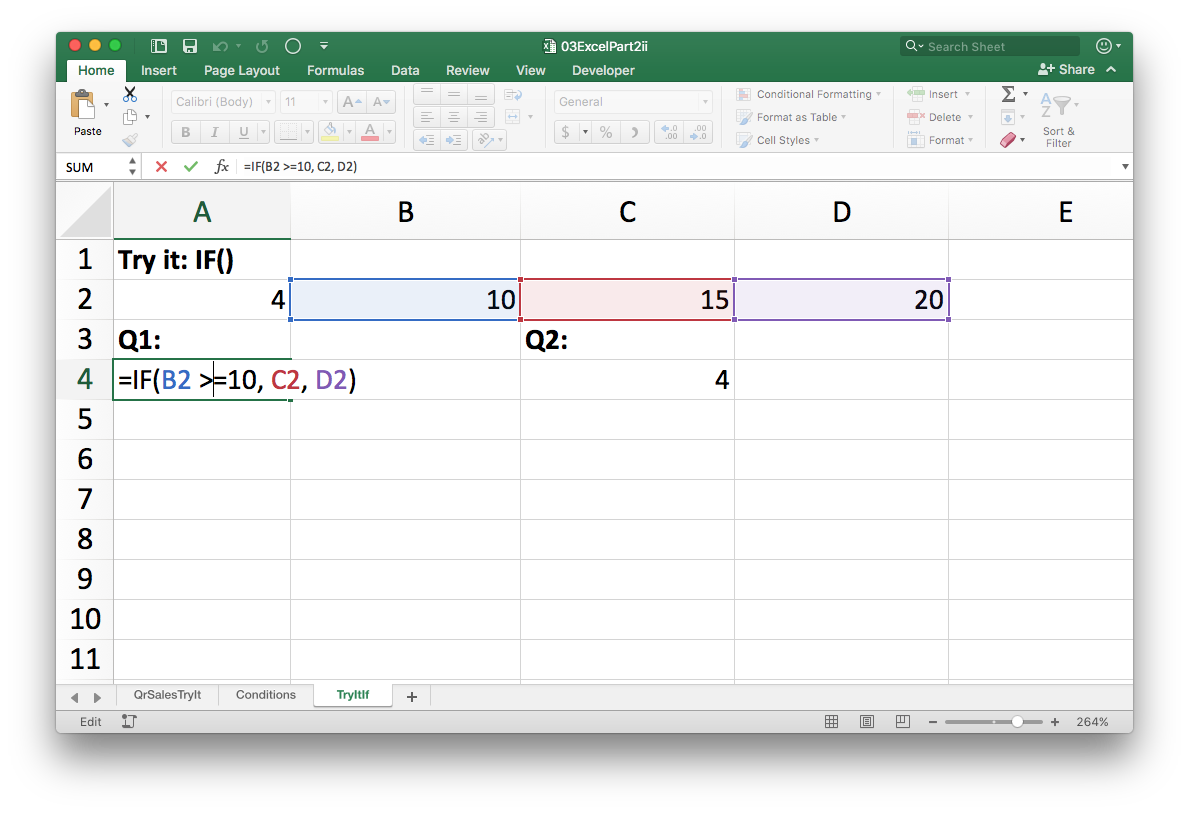
\includegraphics[width=.9\textwidth]{TryItIf2.png}
\end{center}
\end{frame}

\begin{frame}[fragile]{Decision Using {\tt IF()} Question}
  \begin{example}
How many of these statements are TRUE with \cell{A1}=40, \cell{A2}=10?
 \begin{enumerate}
\item \verb|=AND(FALSE(), TRUE())|
\item \verb|=OR(FALSE(), NOT(TRUE()))|
\item \verb|=IF(A1=40, 5, 10)| returns {\tt 10}.
\item \verb|=IF(OR(A1=40,A2>10),1, 2)| returns \tt 2.
\item \verb|=IF(A2=10,IF(A1=40,FALSE()),TRUE())|
 \end{enumerate}
\begin{multicols}{5}
\begin{enumerate}[A)]
\item 0 
\item 1
\item 2
\item 3
\item 4
\end{enumerate}
\end{multicols}
  \end{example} 
\end{frame}


\begin{frame}<handout:0>[fragile]{Decision Using {\tt IF()} Question}
  \begin{block}{Answer:}
How many of these statements are TRUE with \cell{A1}=40, \cell{A2}=10?
 \begin{enumerate}
\item {\color<1->{red}{\verb|=AND(FALSE(), TRUE())|}}
\item {\color<2->{red}{\verb|=OR(FALSE(), NOT(TRUE()))|}}
\item {\color<3->{red}{\verb|=IF(A1=40, 5, 10)| returns {\tt 10}.}}
\item {\color<4->{red}{\verb|=IF(OR(A1=40,A2>10),1, 2)| returns \tt 2.}}
\item {\color<5->{red}{\verb|=IF(A2=10,IF(A1=40,FALSE()),TRUE())|}}
 \end{enumerate}
\begin{multicols}{5}
\begin{enumerate}[A)]
\item \textbf<6>{\textit<6>{{\color<6>{iyellow}{0}}}}
\item 1
\item 2
\item 3
\item 4
\end{enumerate}
\end{multicols}
  \end{block} 
\end{frame}



\begin{frame}{What-If}
\emph{What-If} scenarios help understand different possibilities.\\[1em]
There are three kinds of What-If Analysis tools:
\begin{description}
\item[Scenarios]
\item [Goal Seek]
\item[Data Tables]
\end{description}

A what-if \emph{scenario} is created under {\bf Data} tab then {\bf What-If Analysis} then {\bf Scenario Manager}.\\[1em]
To define a scenario, give it a name and list the cells that will change with this scenario.
\vfill
\begin{alertblock}{Tip}
It is usually a good idea to create a ``Normal" scenario that you can go back to.
\end{alertblock}
\end{frame}

%https://www.ablebits.com/office-addins-blog/2018/09/05/use-goal-seek-excel-what-if-analysis/

\begin{frame}{What-If}
Consider what happens with a cold winter and we predict to sell 50 jackets instead of the normal 15. %\red{BLAH}
\begin{columns}[T] % align columns
\begin{column}{.48\textwidth}
\hspace*{10mm}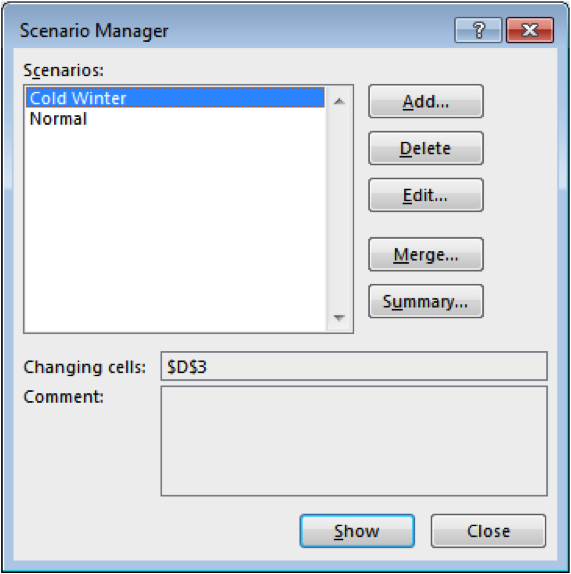
\includegraphics[width=.9\textwidth]{whatif1.png}
\end{column}%
\hfill%
\begin{column}{.48\textwidth}
\hspace*{-6mm}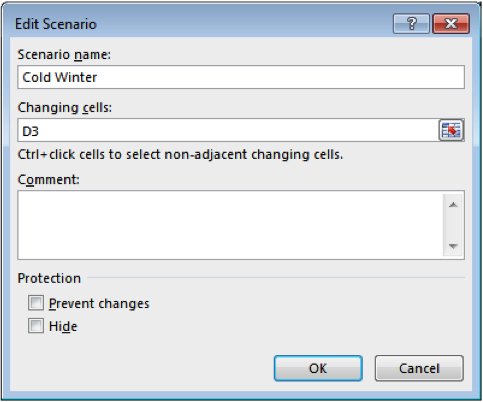
\includegraphics[width=.9\textwidth]{whatif2.png}\\
\hspace*{-6mm}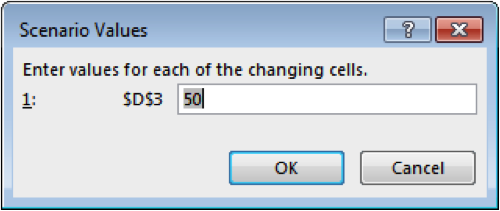
\includegraphics[width=.9\textwidth]{whatif3.png}
\end{column}%
\end{columns}
\end{frame}




\begin{frame}{What-If}
User can easily select scenario and see the result.
\begin{center}
\begin{tikzpicture}
  \node (img1) {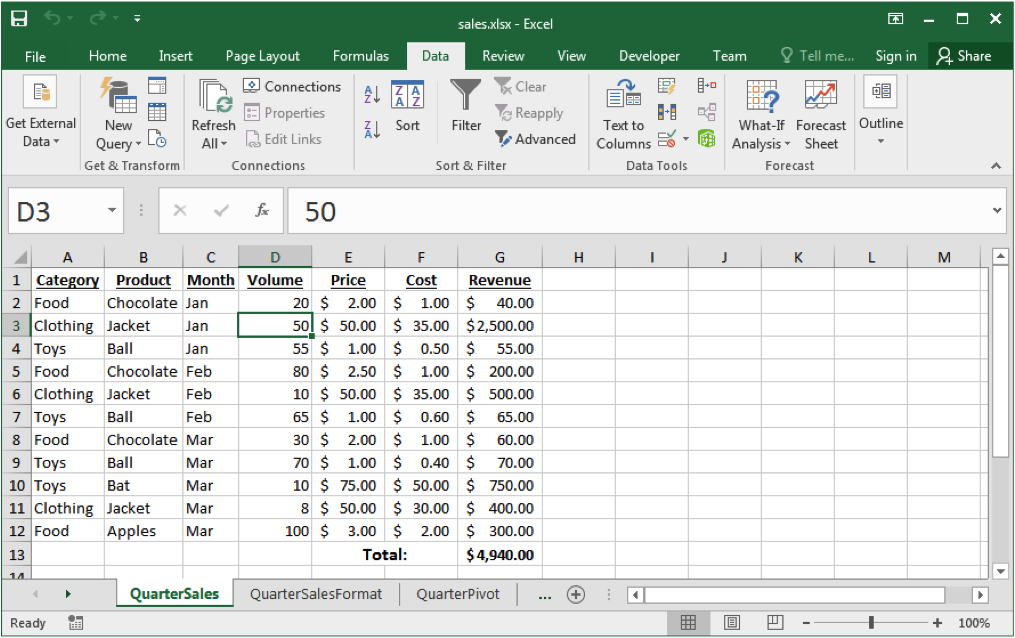
\includegraphics[width=0.9\textwidth]{whatifexcel}};
  
  \node (img2) at (img1.east) [xshift=-2cm] {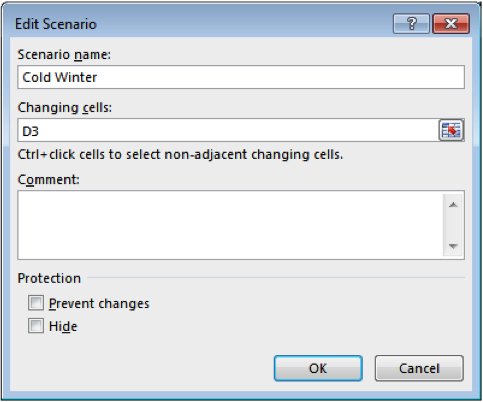
\includegraphics[height=4cm]{whatif2}};
\end{tikzpicture}
\end{center}

\end{frame}

\begin{frame}{Scenario Summary}
\begin{itemize}
\item After creating all of your scenarios, you can create a Scenario Summary Report.
\medskip
\item This report summaries how these scenarios impact a specified {\bf Result Cell}
\medskip
\item For instance, to see how the \textit{Cold Winter} scenario affects total revenue when compared with the \textit{Normal}
\begin{enumerate}
\item go to the {\bf Data} tab then {\bf What-If Analysis} then {\bf Scenario Manager}.  
\item Select {\bf Summary} in the pop up window. 
\item  Select the {\bf Scenario summary} report type and specify the {\bf Result cell} (the value of interest these scenarios will impact). \label{step3}
\end{enumerate}
\end{itemize}
\end{frame}


\begin{frame}{Scenario Summary}
A scenario report will display a summary in table form:
\begin{figure}[htbp]
\begin{center}
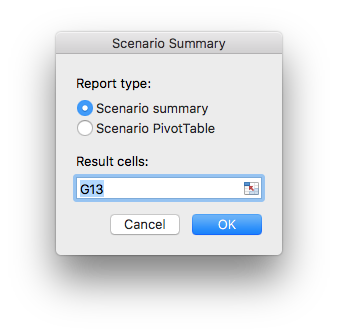
\includegraphics[height=0.4\textwidth]{scwin}
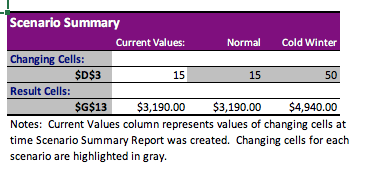
\includegraphics[height=0.3\textwidth]{scsum}
\caption{{\bf Left:} Step \ref{step3} from the previous slide. {\bf Right:} the resulting Scenario Summary  }
\label{default}
\end{center}
\end{figure}

\end{frame}

\begin{frame}{Try it: What-If}
\begin{exampleblock}{Question:} Create a what-if scenario that wherever chocolates are sold, the volume is double than normal. Examine how it affects our total revenue. 
\end{exampleblock}
\begin{center}
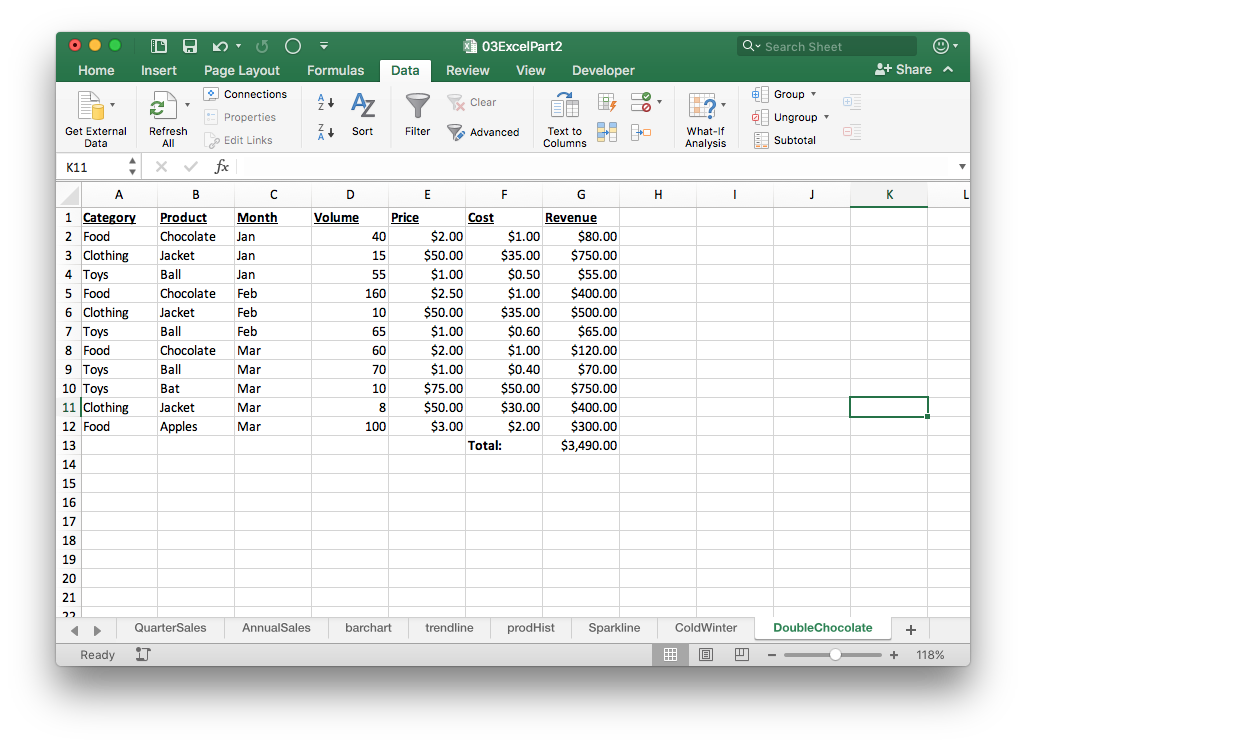
\includegraphics[width=0.8\textwidth]{DoubleChocolate}
\end{center}
\end{frame}


\begin{frame}{Try it: What-If Scenario Challenge}
\begin{exampleblock}{Question:} Create a what-if scenario in which all costs go up by 10\% and volume down by 20\%. 
\end{exampleblock}
\begin{center}
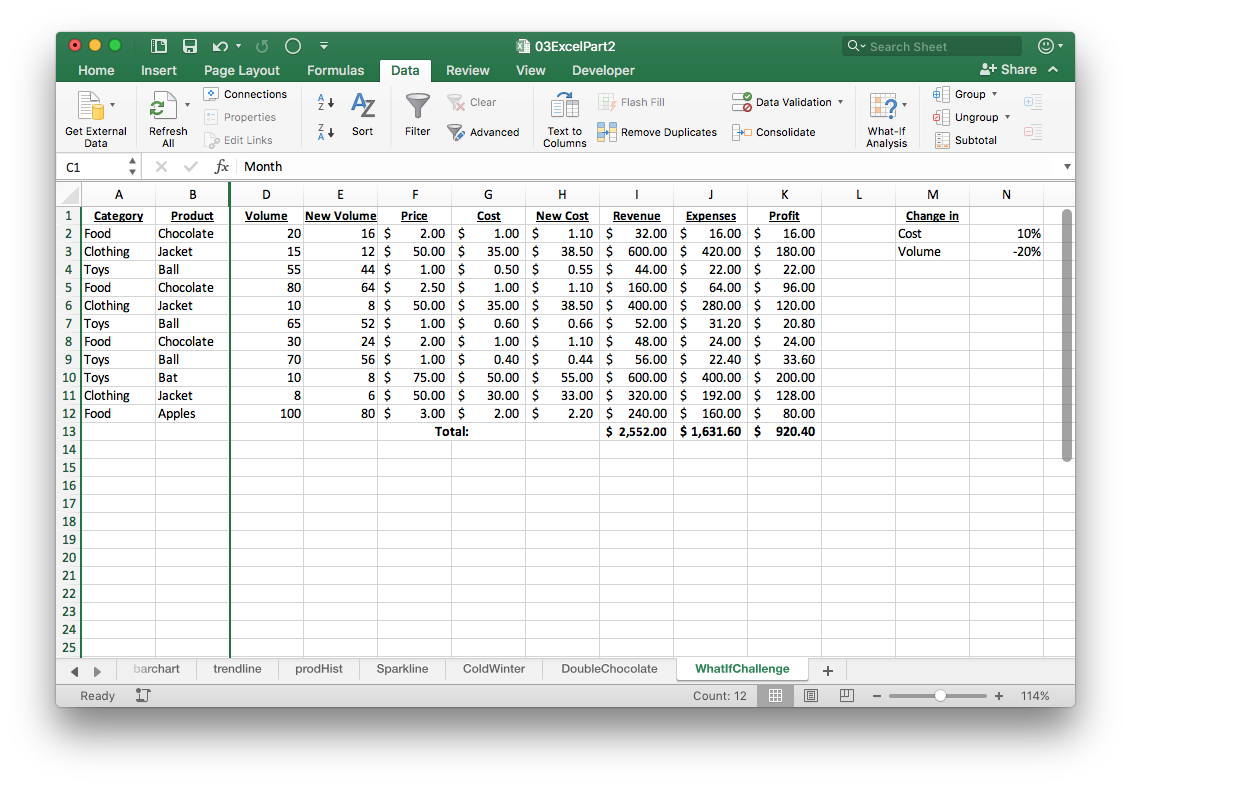
\includegraphics[width=0.8\textwidth]{badcase}
\end{center}
\end{frame}




\begin{frame}{Goal Seek and Solver}
\begin{itemize}

\item Another way to ask Excel "what if" is by using the Goal Seek and Solver tools. \\
\medskip
\item \emph{Goal seek} %({\bf Tools} > {\bf Goal Seek})% excel 2016?
 is used to determine what {\bf value} needs to be in an input cell to achieve a desired result in a formula cell.  \\
 \medskip
\item  \emph{Solver} determines what {\bf values} need to be in multiple input cell{\bf s} to achieve a desired result in a formula cell.  
\begin{itemize}
\item The Solver add-in is similar to Goal Seek, but it can accommodate more variables.
\end{itemize}

\medskip
\item These methods work to achieve a certain goal in the form of a formula \textit{output}, while what-if scenarios looked at changing formula \textit{inputs}.
\end{itemize}
\end{frame}


\begin{frame}{Goal Seek}
\begin{exampleblock}
{}\textcolor{ForestGreen}{\bf Example:} How many balls would we have to sell in January to have total revenue for first 3 months of \$4000?  
\end{exampleblock}
 \begin{enumerate}
 \item Navigate to the {\bf Data} tab, click {\bf What-If Analysis}, and then click {\bf Goal Seek}.
 \item In the {\bf Set cell} box, enter the reference for the cell that contains the formula that you want to resolve, ie. \cell{G13}.

\item In the {\bf To value} box, type the formula result that you want. eg. 4000

\item In the {\bf By changing} cell box, enter the reference for the cell that contains the value that you want to adjust, ie, \cell{D4}
 \end{enumerate}

 \end{frame}


\begin{frame}{Goal Seek}
\begin{center}
%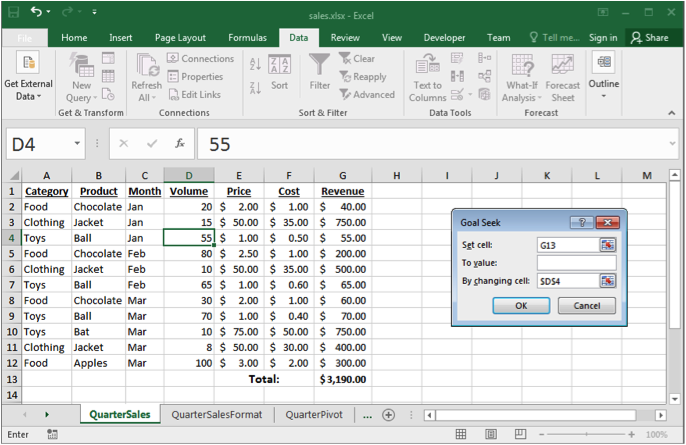
\includegraphics[width=.8\textwidth]{GoalSeek}
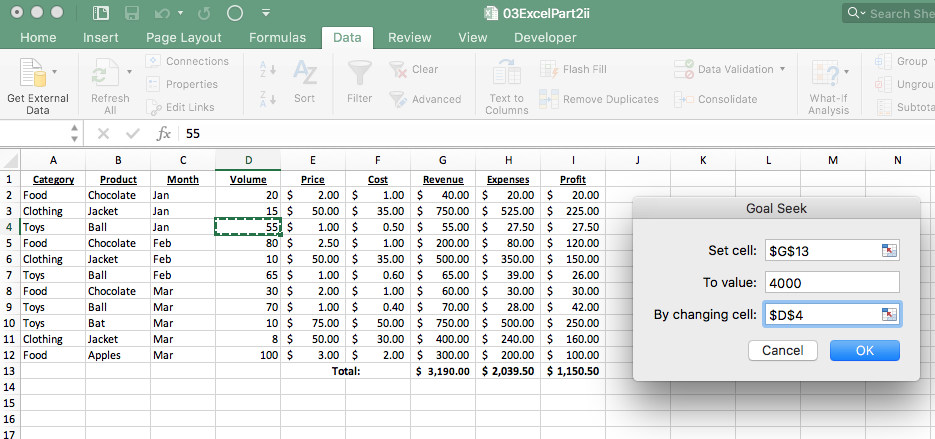
\includegraphics[width=.99\textwidth]{GoalSeek1}
\end{center}
\end{frame}

\begin{frame}{Goal Seek}
\begin{block}
{}\blue{\bf Answer:} How many balls would we have to sell in January to have total revenue for first 3 months of \$4000?  
{\bf Answer: 865}	
\end{block}
\begin{center}
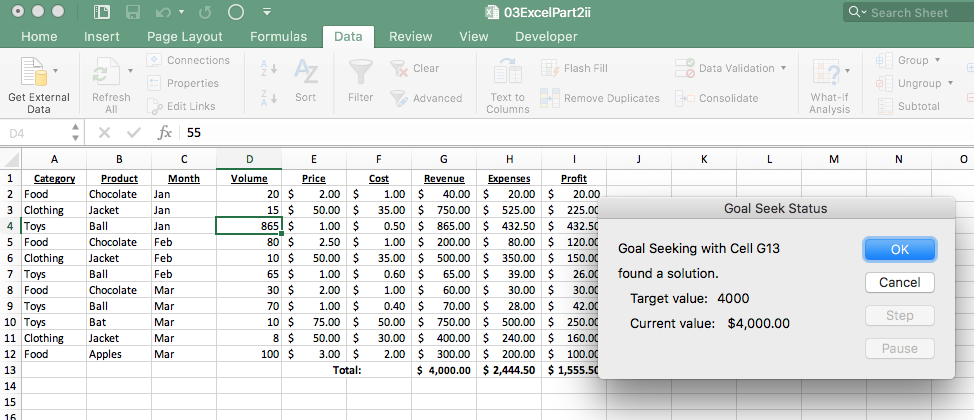
\includegraphics[width=.99\textwidth]{GoalSeek2}
\end{center}
\end{frame}

\begin{frame}{Add ons}
\begin{itemize}
\item Goal Seek only allows a single input value, that is, we can only specify a single cell under the {\it By changing cell} field.
\medskip
\item In order to specify more than one input value we should instead use the Solver.
\medskip
\item To use the Solver Add-in, however, you first need to load it in Excel (\href{https://support.office.com/en-us/article/load-the-solver-add-in-in-excel-612926fc-d53b-46b4-872c-e24772f078ca\#OfficeVersion=Windows}{click here} for instructions on Windows)

\begin{enumerate}
\item On the {\bf Tools} menu, select {\bf Excel Add-Ins}.
\item Select the {\bf Solver Add-in} check box from the Add-Ins available box.
\begin{center}
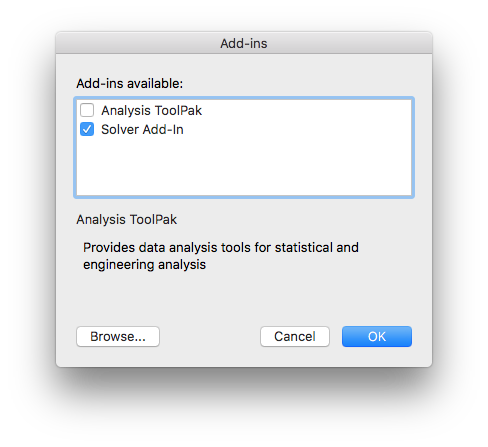
\includegraphics[width=0.25\textwidth]{solveraddin}
\end{center}

%If Solver Add-in is not listed in the Add-Ins available box, click Browse to locate the add-in.

%If you get a prompt that the Solver add-in is not currently installed on your computer, click Yes in the dialog box to install it.

\end{enumerate}
\item After you load the Solver add-in, the Solver button is available on the Data tab.
\end{itemize}
\end{frame}

\begin{frame}{\href{https://support.office.com/en-us/article/define-and-solve-a-problem-by-using-solver-5d1a388f-079d-43ac-a7eb-f63e45925040}{Solver}}
\begin{itemize}
\item Like Goal seek, Solver can be used to determine what values need to be changed to achieve a desired result.  Unlike Goal seek, we can accommodate \textit{multiple} cell values changing.
\medskip
\item In addition, rather than setting our desired result (called the objective cell) to a specific number, we could use Solver to find an optimal (maximum or minimum) value for a formula in one cell subject to certain constraints. 
\medskip
\item Solver works with a group of cells, called decision variables.
\begin{itemize}
\item These cells are necessarily inputs to the objective cell.
\item Solver adjusts these decision variable in order to obtain the desired result in your objective cell.
\end{itemize}

\end{itemize}

\end{frame}


\begin{frame}{Solver Example}
\begin{itemize}
\item For example, lets assume that our final grades are calculated using the following breakdown:
\begin{table}[htdp]
\begin{center}
\begin{tabular}{|c|c|}
\hline
Assignments&10\%\\
Midterm 1& 25\%\\
Midterm 2& 25\%\\
Exam & 40\%\\
\hline
\end{tabular}
\end{center}
\label{default}
\end{table}%
\item Let's assume we've already received 90\% on the assignment component, 65\% on midterm 1, and only midterm 2 and the  exam remain.
\medskip
\item Let's use Solver to determine a scenario in which our resulting final grade would be 75\%.
\medskip
\end{itemize}
\end{frame}

\begin{frame}{Solver Example}
 Consider the \textit{Solver} starter worksheet on {\bf 03ExcelPart2ii.xlsx}
\begin{center}
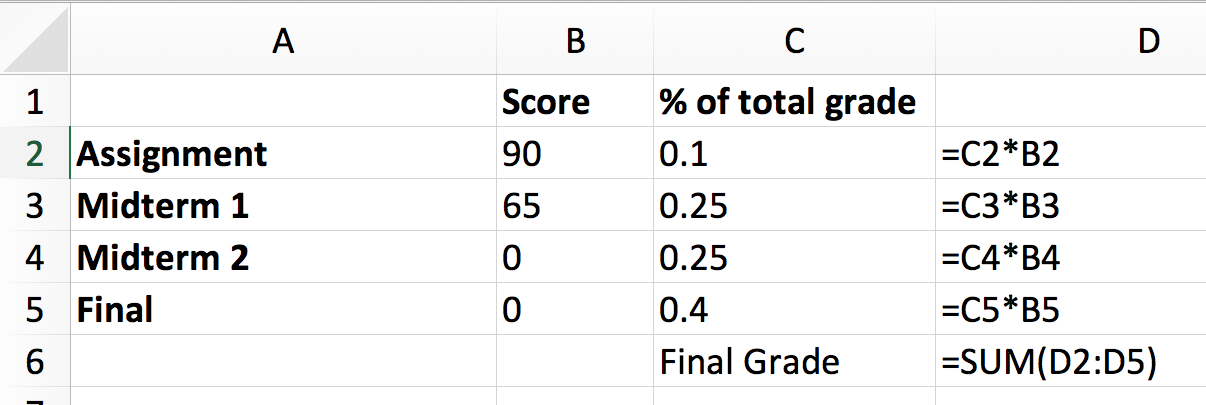
\includegraphics[height=0.3\textwidth]{solverF}
\end{center}
\begin{itemize}
\item Our final grade stored in \cell{D6} is our objective cell.  
\item \cell{B3} and \cell{B5} will be our decision variables.
\item Notice how the calculation of \cell{D6} depends on \cell{B4} and \cell{B5}.
\end{itemize}
\end{frame}

\begin{frame}{Solver Example}
\begin{itemize}
\item Navigate to the {\bf Data} tab and click on the Solver button.
\begin{center}
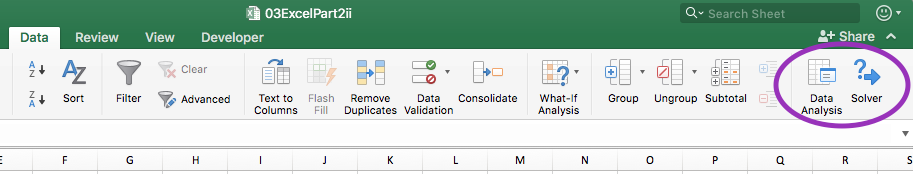
\includegraphics[width=0.9\textwidth]{addins}
\end{center}
\item Specify the objective cell, decision variables and any constraints in the the  pop-up window.
\medskip
\item For this example our only constraints is that  \cell{B3} and \cell{B5} must be $\leq$ 100 and $\geq$ 0.
\end{itemize}
{\bf Sidenote} other constraints include:
\begin{description}
\item[int] Restricting cells to be an integer,
\item[bin] Restricting cells to be a binary digit (either 0 or 1)
\item[dif] Restrict cells to contain different (i.e. non-identical) value
\end{description}
\end{frame}


\begin{frame}{Solver Example}
\begin{center}
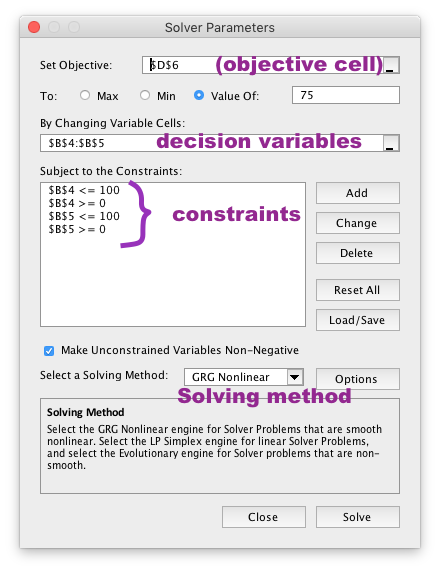
\includegraphics[height = 0.8\textheight]{solverparameters}
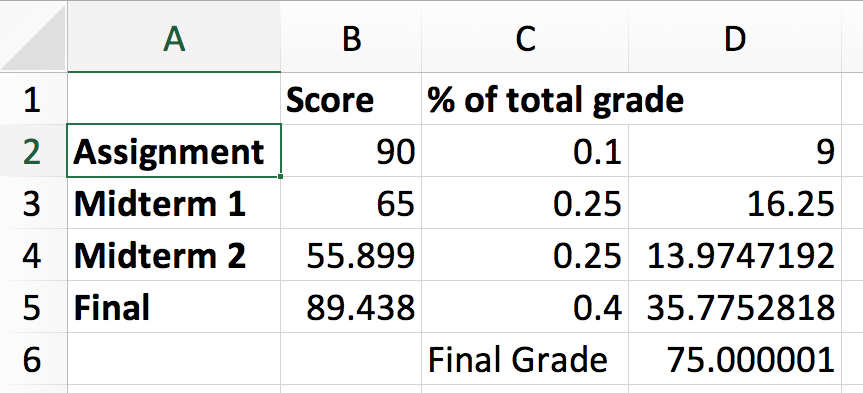
\includegraphics[width = 0.5\textwidth]{solverresult}
\end{center}

\end{frame}


\begin{frame}{Solver}
You may have noticed that there are three different solving methods using solver (as chosen in the {\bf Select a Solving Method} drop-down menu:
\begin{enumerate}
\item       GRG Nonlinear
\item       Simplex LP
\item  Evolutionary.
\end{enumerate}
\medskip
A description of these methods are provided directly below the drop-down menu with further options available by clicking the {\bf Options} button located to the right of this drop-down menu.\\
\medskip
If you are unsure which one to use, it is usually best to select the GRG Nonlinear engine.
\end{frame}





\begin{frame}{What-If Clicker Question}
  \begin{example}
 How many of the following statements are TRUE?
 \begin{enumerate}
\item We can only change a single cell in using Scenario Manager.
\item We can only change a single cell in using Goal Seek.
\item We can only change a single cell in using Solver.
%\item Scenario manager typically changes formula inputs, while Goal Seek and Solver aim to change formula outputs.
on the fitted line.
 \end{enumerate}
\begin{multicols}{4}
\begin{enumerate}[A)]
\item 0 
\item 1
\item 2
\item 3
\end{enumerate}
\end{multicols}
  \end{example} 
\end{frame}

\begin{frame}<handout:0>{What-If Clicker Question}
  \begin{block}{Answer:}
 How many of the following statements are TRUE?
 \begin{enumerate}
\item {\color<1->{red}{We can only change a single cell in using Scenario Manager.}}
\item {\color<2->{ForestGreen}{We can only change a single cell in using Goal Seek.}}
\item {\color<3->{red}{We can only change a single cell in using Solver.}}
%\item {\color<4->{ForestGreen}{Scenario manager typically changes formula inputs, while Goal Seek and Solver aim to change formula outputs.}}
%\item {\color<5->{red}{It is not possible for a field that is a string to be used in VALUES.}}
 \end{enumerate}
\begin{multicols}{5}
\begin{enumerate}[A)]
\item 0 
\item \textbf<4>{\textit<4>{{\color<4>{iyellow}{1}}}}
\item 2
\item 3
\end{enumerate}
\end{multicols}
  \end{block} 
\end{frame}




\begin{frame}{The Analysis ToolPak}
%\red{BLAH try this} \\
\emph{The Analysis ToolPak} is an another Excel \emph{add-in} that has a set of statistical and data analysis tools such as ANOVA, covariance, regression, and t-test.\\[1em]

On a Windows: Analysis ToolPak is not installed by default.
\begin{itemize}
\item To install: {\bf File} $\rightarrow$ {\bf Options} \ra {\bf Add-Ins} 
\item Select {\bf Excel Add-ins} in the {\bf Manage:} box and select {\bf Go} \dots
\item Choose {\bf AnalysisToolPak} and select OK\\[2em]
\end{itemize}


On a mac: {\bf Tools} -->  {\bf Excel Add-ins} select $Analysis Toolpak$\\[2em]

\end{frame}



%\begin{frame}{The Analysis ToolPak}
%You should now see Data Analysis under the Data tab
%\begin{center}
%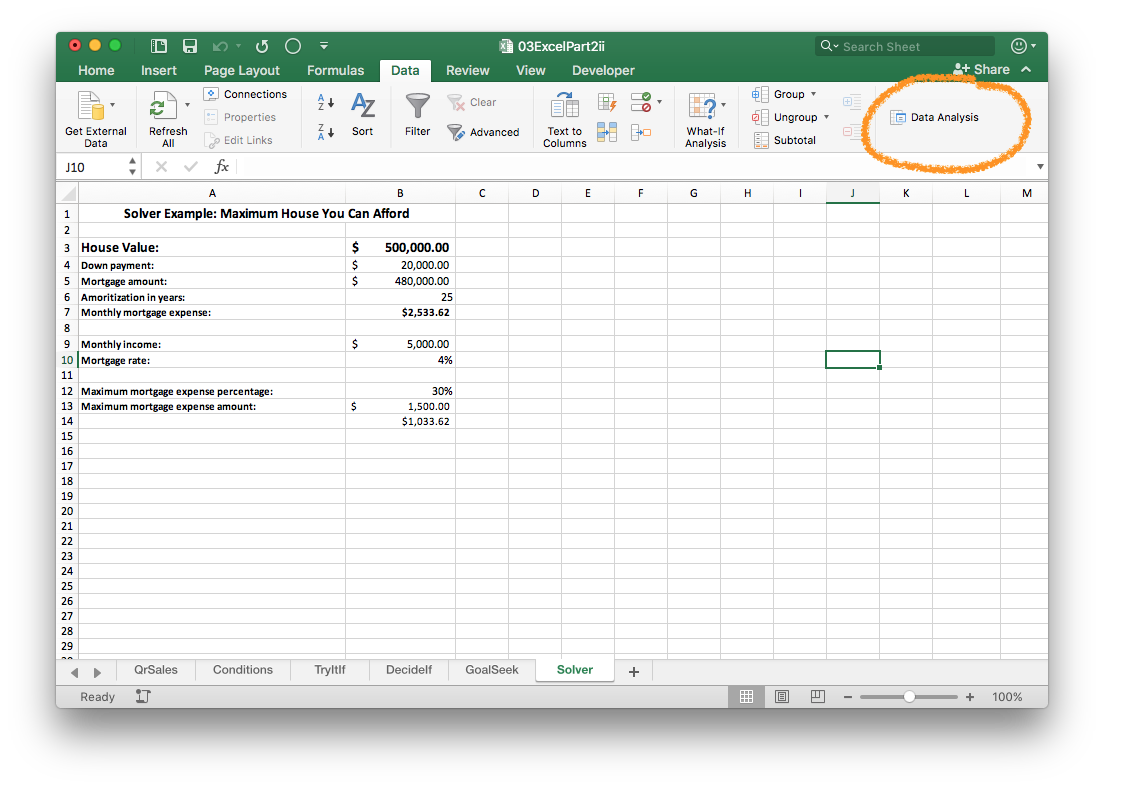
\includegraphics[width=.99\textwidth,valign=t]{toolpack}
%\end{center}
%\end{frame}
%
%\begin{frame}{The Analysis ToolPak}
%For the next example, follow the same steps from the previous two slides to activate the {\bf Solver} Add-in.\\[1em]
%
%\emph{Solver} performs linear programming to maximize or minimize a given function by changing multiple variables subject to constraints.\\[1em]
%
%\end{frame}


\begin{frame}[label=current]{Regression}
\emph{Linear regression} models the relationship between a dependent variable $Y$ and explanatory/independent variable(s) $X$. \\[1em]	
\textit{Simple} linear regression has one explanatory variable, $X$, and can be modelled using the equation
\begin{equation}
Y = \beta_0 +  \beta_1 X +  \epsilon
\end{equation}
\begin{itemize}
\item You can think of $\beta_0$  as the $y$-intercept ($b$) and  $\beta_1$ as the slope ($m$) is an equation for a line $y = m*x + b$ from high school.
\medskip
\item $\epsilon$ denotes the random error about the line which we cannot account for in our model
\end{itemize}
N.B. \emph{Trend lines} are often calculated using linear regression.
\end{frame}



\begin{frame}[label=current]{Regression\footnote{N.B. To learn more on  linear regression, I encourage you to take STAT 121/230 or read \href{https://books.google.ca/books?id=i0DOBQAAQBAJ&printsec=frontcover&dq=Faraway\%27s+Linear+Models+with+R+(2005,+p.+59).\&hl=en\&sa=X\&ved=0ahUKEwinqMbTjq3iAhVhMX0KHedMCnkQ6AEIMjAB\#v=onepage\&q\&f=false}{Faraway's Linear Models with R}}}
\begin{itemize}
\item The technique provides a way to determine linear patterns in the data set.
\medskip
\item The so-called fitted model can be used to:
\begin{enumerate}
\item determine the strength of the relationship between variables $Y$ and $X$ and/or 
\item  predict the outcome variable $Y$ for a new variable $X$.
\end{enumerate}
\medskip
%\item We can use linear models to fit a predictor model on observed data and/or use them to determine the strength of the relationship between $x$ and $y$.\\[1em]
\item To address either of these points, we need the fitted model comprised of the estimates of the regression equation coefficients.
\begin{itemize}
\item  $\hat \beta_0$ and  $\hat \beta_1$ are the estimates for $\beta_0$ and $\beta_1$ respectively.
\item the fitted line is given by $\hat Y =\hat \beta_0 + \hat \beta_1 X$
\end{itemize}
\end{itemize}

%\textit{\footnotesize N.B. To learn more on this linear regression, I encourage you to take STAT 121/230 or read \href{https://books.google.ca/books?id=i0DOBQAAQBAJ&printsec=frontcover&dq=Faraway\%27s+Linear+Models+with+R+(2005,+p.+59).\&hl=en\&sa=X\&ved=0ahUKEwinqMbTjq3iAhVhMX0KHedMCnkQ6AEIMjAB\#v=onepage\&q\&f=false}{Faraway's Linear Models with R}}.

\end{frame}

\begin{frame}[label=current]{Regression in Excel- $R^2$ value}
\begin{itemize}
\item Regarding point 1. Excel regression function that will calculate $R^2$, the coefficient of determination which is a statistical measure of how close the data are to the fitted regression line.
\medskip
\item Mathematically speaking, this is the percentage of the variation in $Y$ that is explained by a linear model. 
\medskip
\item This range of this value is from 0--1.
\begin{itemize} 
\item A value of 0 indicates that the model explains \textit{none} of the variability of the response data around its mean and 
\item a value of 1 indicates that the model explains \textit{all} the variability of the response data around its mean.
\end{itemize}
\end{itemize}
\end{frame}

\begin{frame}{Regression in Excel- $R^2$ value}
\begin{figure}[h]
\begin{center}
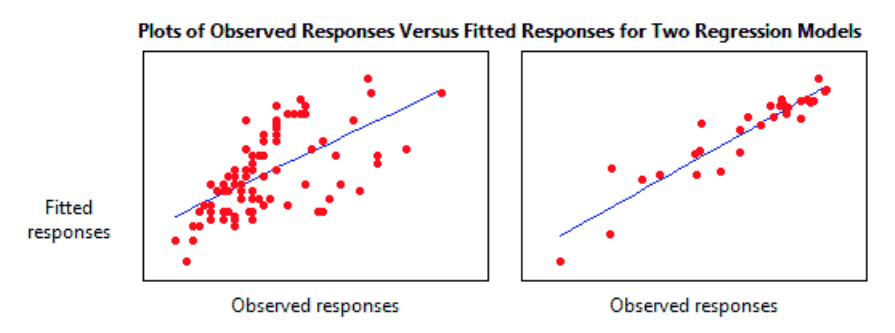
\includegraphics[width=0.85\textwidth]{img/rsquared.png}
\caption{The regression model on the left accounts for 38.0\% of the variance (ie. $R^2 = 0.38$) while the one on the right accounts for 87.4\% (i.e has an $R^2 = 0.874$). Source of image \href{https://blog.minitab.com/blog/adventures-in-statistics-2/regression-analysis-how-do-i-interpret-r-squared-and-assess-the-goodness-of-fit}{here}.}
\label{default}
\end{center}
\end{figure}

\end{frame}




\frame{
\frametitle{Linear Regression assumptions}
The legitimacy of this model depends on the following assumptions:
\begin{enumerate}
\item\textbf{Linearity:} The means of the values of $X$ fall approximately on the straight line $\beta_0 + \beta_1 \, X$ for simple linear regression, fall approximately on the plane  $\beta_0 + \beta_1 \, X_1, \beta_2 \, X_2$ for multiple linear regression, \dots (harder to visual in larger dimensions). 

\item The error terms $\epsilon\overset{\text{i.i.d}}{\sim} N(0, \sigma^2)$. That is:
\begin{itemize}
\item\textbf{Normality:} For each value of the explanatory variable $(X)$ there
is a subpopulation of response variables $(Y)$ that is normally
distributed.\medskip
\item\textbf{Constant variance (homoscedasticity):} All subpopulations have the same standard deviation $\sigma^2$.\medskip
\item\textbf{Independence:} All observations are independent.\medskip
\end{itemize}
\end{enumerate}
N.B. non-constant variance = heteroscedasticity
%{\small Note: No assumptions are needed for the distribution of $X$}
}


\begin{frame}[label=current]{Regression in Excel- Testing Assumptions}
\begin{itemize}
\item To check the {\bf linearity} assumption for simple linear regression, it is always a good idea to plot your data in a \textit{scatterplot}.
\medskip
\item To check the {\bf normality} assumption, we can look at the \textit{Normal Probability Plot} of residuals. 
\begin{itemize}
\item If the data are normal the points should form an approximate straight line. 
\end{itemize}

\medskip
\item The {\bf constant variance} assumption can be assessed using a \textit{residual plot} (where a residual  is the difference between our observed and predicted $y$, i.e. $y_i - \hat y_i$).
\begin{itemize}
%%\item ANOVA table 
\item A `good' residual plot should show no pattern and look like random noise about 0.
%%\item standardized and unstandardized residuals 
\end{itemize}
\medskip
\item A pattern in the residual plot may suggests a violation of the {\bf independence} assumption.  Reason for this may include:
\begin{itemize}
\item Time series data,  related individuals (same family, same household).
\end{itemize}


\medskip
\end{itemize}
\end{frame}


\begin{frame}[label=current]{Testing Assumptions Using Residual Plots}
\begin{figure}[htbp]
\caption{Image taken from \href{https://books.google.ca/books?id=i0DOBQAAQBAJ&printsec=frontcover&dq=Faraway\%27s+Linear+Models+with+R+(2005,+p.+59).\&hl=en\&sa=X\&ved=0ahUKEwinqMbTjq3iAhVhMX0KHedMCnkQ6AEIMjAB\#v=onepage\&q\&f=false}{Faraway's Linear Models with R (2005, p. 59).} }
\begin{center}
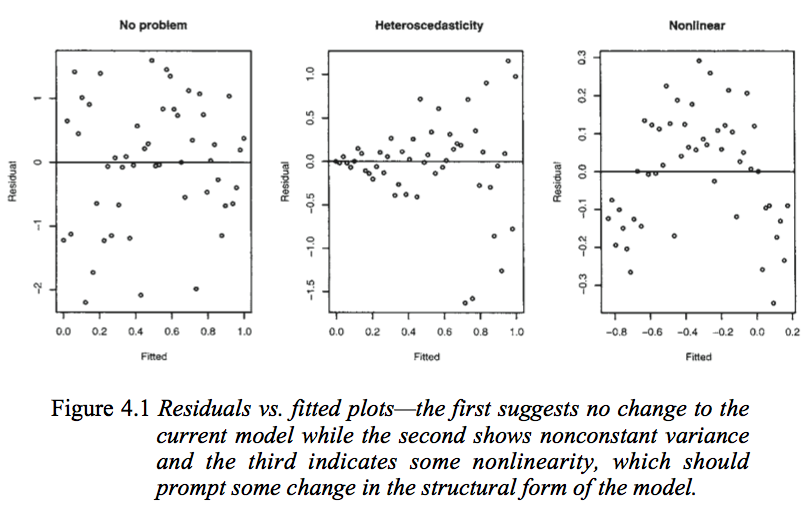
\includegraphics[width=0.9\textwidth]{img/resplot.png}
\label{default}
\end{center}
\end{figure}
\end{frame}

\begin{frame}[label=current]{Testing Assumptions Using Normal Probability Plots}
\begin{figure}[htbp]
\caption{The points on a ``good" normal probability plots should fall approximately on a straight line.   Images taken from \href{https://www.slideshare.net/saqibshahzad26/26-assumptions}{SlideShare} }
\begin{center}
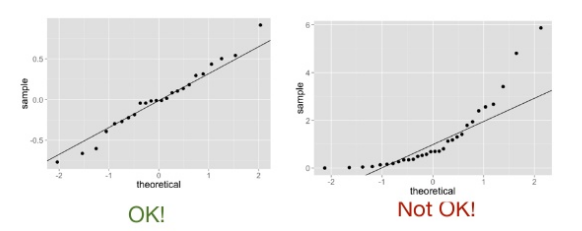
\includegraphics[width=0.8\textwidth]{img/ppplot}\\
\includegraphics[width=0.8\textwidth]{img/notok}
\label{default}
\end{center}
\end{figure}
\end{frame}






\begin{frame}[label=current]{Regression in Excel}
\begin{exampleblock}{
Example:} Given a data set of car weight and acceleration, determine if there is any relationship between them.\end{exampleblock}

\begin{center}
\includegraphics[height=.45\textheight]{avsw2}
\end{center}
% For ease of use, the independent variable should be in the left column as this column is going to be plotted on the x axis. The dependent variable (the one affected by the independent variable) should be in the right column, and it will be plotted on the y axis.
% https://www.ablebits.com/office-addins-blog/2018/10/03/make-scatter-plot-excel/
Scatterplot shows weak relationship with no strong patterns, and we would expect to see this shown in the regression analysis.
\end{frame}



\begin{frame}[label=current]{Regression in Excel}
Regression computes constants m and b in formula:
\begin{center}
\yellow{acceleration} = $m$*\textcolor{ForestGreen}{weight} +$b$ = $\beta_1$*\textcolor{ForestGreen}{weight} +$\beta_0$
\end{center}
Acceleration is the \yellow{dependent variable} and weight is the \textcolor{ForestGreen}{independent variable}\\[1em]
\begin{center}
\includegraphics[height=.45\textheight]{Regression2}
\end{center}
To start select, {\bf Data Analysis} from the {\bf Data} tab  and then select {\bf Regression} and {\bf OK} . 
\end{frame}

\begin{frame}[label=current]{Regression Example Settings}
\begin{columns}[T] % align columns
\begin{column}{.6\textwidth}
\includegraphics[height=.6\textheight]{RegressionSettings}
\end{column}%
\hfill%
\begin{column}{.5\textwidth}
Settings:
\begin{itemize}
\item Response (dependent) data for the Input Y Range
\item Columns for the explanatory (independent) data (X Range). 
\item For residual information select, Residuals, Standardized Residuals, and Residual Plots from the Residuals section. 
\end{itemize}
\end{column}%
\end{columns}
\end{frame}



\begin{frame}
\begin{center}
\includegraphics[height=.6\textheight]{regpopup}
\end{center}
If you select the column headers, be sure to select the {\bf Labels} options to ensure they are treated as meta-data.\\
\medskip
Notice that many of the features regarding the residuals are not selected by default.
\end{frame}



%\begin{frame}[label=current]{Regression Example Results}
%\begin{center}
%\includegraphics[width=.8\textwidth]{RegRes}
%\end{center}
%\end{frame}

\begin{frame}[label=current]{Regression Example Results}
\begin{center}\includegraphics[width=.8\textwidth]{RegressionResults}
\end{center}
All of the output is put into a new sheet.  Read the values off of the table and form the regression equation: 
\begin{center}
acceleration = -0.001353896*weight + 19.57266581
\end{center}
As one might expect, a weak relation is found as reflected by the  $R^2$ value 
\begin{itemize}
\item Only 17.4\% of the variation in weight is explained by acceleration. 
\end{itemize}

\end{frame}

\begin{frame}[label=current]{Regression Example Results (cont.)}
Below the previous tables are the predicted y values (from the regression equation) as well as the residuals and standardized residuals (residuals divided by their standard deviation). 
\begin{center}
\includegraphics[width=.75\textwidth]{RER1}
\end{center}
\end{frame}



\begin{frame}[label=current]{Regression Example Results (cont.)}
\begin{center}
\includegraphics[width=.75\textwidth]{RER1a}
\end{center}
\begin{align*}
\text{eg. }X_1=3504, \text{ hence } \hat Y_1 &= -0.001353896*weight + 19.57266581 \\
&-0.001353896*3504 + 19.57266581\\
& = 14.82861423 \text{ (with some rounding error)}
\end{align*}
\end{frame}


\begin{frame}[label=current]{Regression Example Results (cont.)}
\begin{center}
\includegraphics[width=.75\textwidth]{RER1b}
\end{center}
The observed acceleration for observation 1 was $Y_1=12$.  To calculated the residual, we subtract the true value $Y_1$ from the predicted value $\hat Y_1$
\begin{align*}
e_1 \text{(the residual of obs. 1)} &= Y_1 - \hat Y_1\\
&= 12 - 14.82861423 \\
& = -2.828614226 \text{ (rounding error)}
\end{align*}
\end{frame}



\begin{frame}[label=current]{Regression Example Results (cont.)}
 All plots are placed to the right of the charts.\\ 
\begin{center}
\includegraphics[height=.4\textheight]{RER2}\includegraphics[height=.4\textheight]{normalpp}
\end{center}
\begin{itemize}
\item This is a ``good" residual plot since it shows no obvious pattern and  points are  symmetrically distributed  around a horizontal line with a roughly constant variance.
\item The Normal Probability Plot shows some curvature in the tails indicating that the residuals are showing some departure from normality. 
\end{itemize}
\end{frame}

\begin{frame}[label=current]{Regression Example Results (cont.)}
As you can see, these are also the results obtained when fitting a trendline to the original scatterplot
\begin{center}
\includegraphics[width=.9\textwidth]{trendlineinfo}
\end{center}

\end{frame}



\begin{frame}[label=current]{Try It: Regression}
\begin{exampleblock}
{Question:} Perform a regression analysis between weight (dependent) and displacement (independent) variable.
\end{exampleblock}
\begin{center}
\includegraphics[width=.7\textwidth]{WvsD}
\end{center}
\end{frame}


\begin{frame}
  \begin{example}
 How many of the following statements are TRUE?
 \begin{enumerate}
\item Regression can only be used when we have one dependent variable $Y$ and one explanatory variable $X$.
\item No assumptions are needed for the distribution of $X$ in order to fit a linear regression model.
\item Residual plots may be used to test linear model assumptions.
\item A $R^2$ value of 1 means that all points in our data set lie exactly on the fitted line.
 \end{enumerate}
\begin{multicols}{5}
\begin{enumerate}[A)]
\item 0 
\item 1
\item 2
\item 3
\item 4
\end{enumerate}
\end{multicols}
  \end{example} 
\end{frame}

\begin{frame}<handout:0>{What-If and Pivot Tables Question}
  \begin{block}{Answer:}
 How many of the following statements are TRUE?
 \begin{enumerate}
\item {\color<1->{red}{Regression can only be used when we have one dependent variable $Y$ and one explanatory variable $X$.}}
\item {\color<2->{ForestGreen}{No assumptions are needed for the distribution of $X$ in order to fit a linear regression model.}}
\item {\color<3->{ForestGreen}{Residual plots may be used to test linear model assumptions.}}
\item {\color<4->{ForestGreen}{A $R^2$ value of 1 means that all points in our data set lie exactly on the fitted line.}}
%\item {\color<5->{red}{It is not possible for a field that is a string to be used in VALUES.}}
 \end{enumerate}
\begin{multicols}{5}
\begin{enumerate}[A)]
\item 0 
\item 1
\item 2
\item \textbf<4>{\textit<4>{{\color<4>{iyellow}{3}}}}
\item 4
\end{enumerate}
\end{multicols}
  \end{block} 
\end{frame}



\begin{frame}[label=current]{Conclusion}
\emph{Spreadsheets} are general purpose tools for data analysis that consist of a table of cells which contain data and formulas.\\[1em]
Formulas contain data values, cell references, and functions.
\begin{itemize}
\item Aggregate functions summarize multiple data values into a single value.
\item Functions exist for statistics, string manipulation, lookup/indexing, and decisions.
\end{itemize}
Spreadsheets provide tools for data sorting, filtering, visualization using charts, and summarization (pivot tables).  \\[1em]
Also contain tools for what-if scenarios, goal seek, linear solvers, and statistical analysis tools.
\end{frame}

\begin{frame}{Objectives}
\begin{itemize}
\item Explain what a spreadsheet is.
\item Explain how cells are addressed in a spreadsheet.
\item List some of the ways to select cells in a spreadsheet.
\item Define and explain: formula, function, argument, concatenation
\item Use these functions: concatenate, lookup, index
\item Explain the difference between an absolute and relative address.
\item Explain how an aggregate function works.  List some examples.
\item Explain how to use conditional formatting.
%\item Explain how spreadsheets can be used as a database. 
\item  Use sorting and filtering.
\item Be able to create and edit charts and use chart features: trendlines, sparklines
\item Explain the usefulness of: what-if scenarios, goal seek, solver
\item Use and create pivot tables and charts.
\item Evaluate and create conditions. Use IF() to make decisions.
\end{itemize}
\end{frame}



\end{document}

